\documentclass[twoside, 12pt]{iiser-thesis}

%%%%%%%%%%%%%%%%%%%
% Packages/Macros %
%%%%%%%%%%%%%%%%%%%
\usepackage{fullpage}
\usepackage{amssymb,latexsym,amsmath}     % Standard packages
\usepackage{graphicx}
\graphicspath{ {./figures/} }
\usepackage{authblk}
\usepackage{dsfont}
\usepackage{amsthm}
\usepackage{color}
\usepackage{float}
\usepackage[breaklinks=true]{hyperref}
\usepackage[style=apa,
			sorting=nyt,
			date=year,
			bibencoding=utf8,
			isbn=false,
			eprint=false,
			dashed=false,
			uniquelist=false,
			maxbibnames=10,
			minbibnames=1,
			maxcitenames=2,
			uniquename=init,
			giveninits=true,
			useprefix=false,
			minsortnames=1,
			maxsortnames=2]{biblatex}
\renewcommand{\cite}{\parencite}
\bibliography{References}
\setlength{\parskip}{1em}
\usepackage{xurl}
\usepackage{longtable}
\usepackage{caption}
\usepackage{subcaption}
\usepackage{multirow}
%
% please place your own definitions here and don't use \def but
% THEOREM Environments ---------------------------------------------------

\newtheorem{theo}{{\bf{Theorem}}}[section]
\newtheorem{prop}[theo]{{\bf Proposition}}
\newtheorem{lem}[theo]{{\bf Lemma}}
\newtheorem{coro}[theo]{{\bf Corollary}}
\newtheorem{ex}{{\bf Example}}
\newtheorem{exer}{{\bf Exercise}}
\newtheorem{rem}{{\bf Remark}}[section]
\newtheorem{rems}[rem]{{\bf Remarks}}
\newtheorem{remark}[rem]{Remark}
\newtheorem{defi}{{\bf Definition}}[section]
\newtheorem{defn1}[defi]{Definition}
\newtheorem{defs}[defi]{{\bf Definitions}}
\newtheorem{notation}{{\bf Notation}}[section]
%\newtheorem{mypar}{{\bf }}[section]
%\newcommand{\skp}{\vspace{\baselineskip}}
%%\newcommand{\qed}{\hfill\rule{1.6mm}{1.6mm}}
%\renewcommand{\proof}{\noindent{\bf Proof.\ }}
%\newcommand{\no}{\nonumber}
%\newcommand{\noi}{\noindent}
%\newcommand{\txt}{\textrm}
%\newcommand{\pa}{\partial}
%\newcommand{\ds}{\displaystyle}
%\newcommand{\RR}{\mathbb{R}}
%\newcommand{\si}{\sigma}
%\newcommand{\al}{\alpha}
%\newcommand{\la}{\lambda}
%\newcommand{\La}{\Lambda}
%\newcommand{\calF}{\mathcal{F}}
%\newcommand{\eps}{\varepsilon}
%\newcommand{\ph}{\varphi}
%\newcommand{\sig}{\sigma}
%\newcommand{\tab}{\hspace*{0.3in}}
%\newcommand{\Tab}{\hspace*{1.0in}}
%\newcommand{\vf}{\varphi}
%\newcommand{\del}{\frac{\partial}{\partial t}}
%\newcommand{\vp}{\varepsilon}


\catcode`\@=11
\catcode`\@=12


%%%%%%%%%%%%
% Document %
%%%%%%%%%%%%
%\setcounter{chapter}{-1}

\title{Studying effects of competition on adaptive therapy}


\author{Harshavardhan BV }
\coordinator{Coordinator} \supervisor{Prof. Sutirth Dey} \sdesignation{Professor}
\department{Department of Biology} \reader{Dr. M.S. Madhusudhan}
%\reader{Reader 2}
\dedication{This thesis is dedicated to ?}
\graduationyear{2021}
\academicyear{2020-2021}
\graduationmonth{July}
\def \@bd@lot{0}

\thesisabstract{ Write your  abstract here
}
\acknowledgments{Not more than 250 words}

\begin{document}
	\thesisfront

\section{Introduction}

\begin{frame}{Conventional and adaptive Therapy}
  \begin{columns}
    \begin{column}{0.45\textwidth}
      \begin{itemize}
        \item Conventional therapy @ MTD $\rightarrow$\\
        $\downarrow$ tumour burden \cite{Frei}
        \item Heterogenous sensitivity $\rightarrow$\\
        sens. $\times$ $\rightarrow$ resst. \cite{Scott}
        \item AT = $\downarrow$ , $\sim$ dose $\rightarrow$ sens. $\checkmark$ \cite{Gatenby}
        \item Drug holiday - sens. $\rightarrow\ \downarrow$ resst.
        \item AT outcome $\leftarrow$ competition
      \end{itemize}
    \end{column}
    \begin{column}{0.55\textwidth}
      \begin{figure}[h]
        \centering
        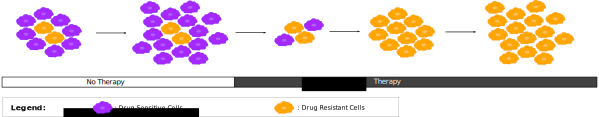
\includegraphics[width=\textwidth]{compe_release}
        \caption{Competitive release under SOC}
      \end{figure}
      \begin{figure}[h]
        \centering
        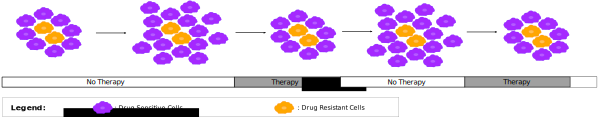
\includegraphics[width=\textwidth]{at}
        \caption{Control under AT}
      \end{figure}
    \end{column}
  \end{columns}
\end{frame}

\begin{frame}{System of study}
  \begin{itemize}
    \item Castration-Resistant Prostate Cancer (CRPC)
    \item AR pathway: prostate cells $\rightarrow$ cancer \cite{Heinlein}
    \item Therapy: ADT + Abiraterone
  \end{itemize}
  \begin{table}
    \centering
    \begin{tabular}{|l|c|c|c|c|}
    \hline
    Cell type & Test. dependent & Test. Producing & Ab. sensitive & Mechanism \\
    \hline
    $T^+$ & Yes & No & Yes & N/A \\
    $T^p$ & Yes & Yes & Yes & Cholesterol $\xrightarrow{CYP17\alpha}$ Test.\\
    $T^-$ & No & No & No & AR $\mu^n$\\
    \hline
    \end{tabular}
  \end{table}
\end{frame}

\begin{frame}{System of equations}
  \begin{columns}
    \begin{column}{0.45\textwidth}
      \begin{itemize}
        \item Logistic framework w/ dynamic carrying capacity $\approx$ env. condn.
        \item Environment = resource = $\{O_2,test\}$
        \item No $\mu^n$, no spatial structure, well mixed
        \item Defined $\mathbb{R}_{\geq 0}$, $y_i < 1 =$ extinction
      \end{itemize}
      \begin{figure}[h]
        \centering
        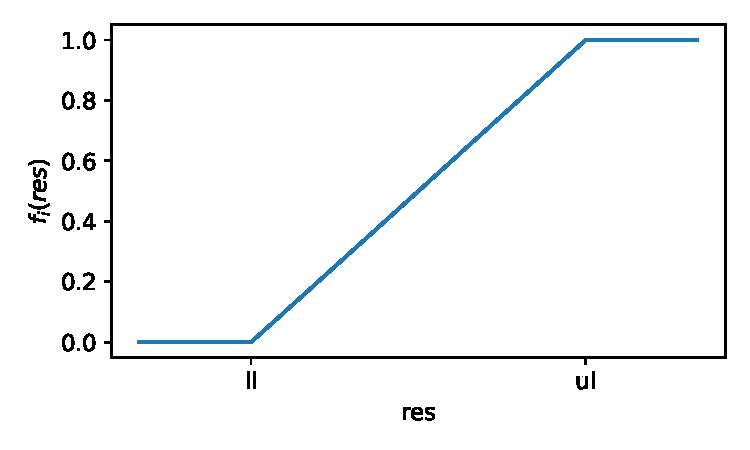
\includegraphics[width=\textwidth]{f_res}
        \caption{$f_i(res)$}
      \end{figure}
    \end{column}
    \begin{column}{0.55\textwidth}
      \begin{equation}
        \frac{dy_i}{dt} = r_i y_i (1 - \frac{\sum_j y_j}{1 + K_{i,max} f_i(O_2) f_i(test)} )- \delta_i y_i
        \label{celleq}
      \end{equation}
      \begin{equation}
        \frac{dO_2}{dt} = p_{O_2} - \sum_i \mu_{O_2,i} y_i - \lambda_{O_2} O_2
        \label{o2eq}
      \end{equation}
      \begin{equation}
        \frac{dtest}{dt} = p_{test} y_{T^p} - \sum_i \mu_{test,i} y_i - \lambda_{test} test
        \label{testeq}
      \end{equation}
      \begin{equation}
        f_i(res) = \begin{cases}
          1 &\text{if } ul_{res,i} \leq res\\
          \frac{res-ll_{res,i}}{ul_{res,i}-ll_{res,i}} &\text{if } ll_{res,i} < res < ul_{res,i}\\
          0 &\text{if } res \leq ll_{res,i}\\
        \end{cases}
        \label{freseq}
      \end{equation}
      $i \in \{T^+,T^p,T^-\}$ and $res \in \{O_2,test\}$.
    \end{column}
  \end{columns}
\end{frame}


\chapter{Methods}

\section{System of Equations}
The system of study was modelled using coupled Ordinary Differential Equations (ODEs). The model is based on a logistic framework modified with a dynamic carrying capacity that depends on the environmental conditions. The ``environment" consists of the resources, oxygen and testosterone which have their own equations for production and consumption. We make the simplifying assumption that every other resource required by cells are present in non-limiting concentrations. Additionally, the cell types were assumed to not mutate and hence cannot change their types. No spatial structure is considered and the system is assumed to be well mixed and the resource available in bulk for all the cells. The ODEs are given below:

For $i \in \{T^+,T^p,T^-\}$ and $res \in \{O_2,test\}$

\begin{equation}
  \frac{dy_i}{dt} = r_i y_i (1 - \frac{\sum_j y_j}{1 + K_{i,max} f_i(O_2) f_i(test)} )- \delta_i y_i
  \label{celleq}
\end{equation}
\begin{equation}
  \frac{dO_2}{dt} = p_{O_2} - \sum_i \mu_{O_2,i} y_i - \lambda_{O_2} O_2
  \label{o2eq}
\end{equation}
\begin{equation}
  \frac{dtest}{dt} = p_{test} y_{T^p} - \sum_i \mu_{test,i} y_i - \lambda_{test} test
  \label{testeq}
\end{equation}
\begin{equation}
  f_i(res) = \begin{cases}
    1 &\text{if } ul_{res,i} \leq res\\
    \frac{res-ll_{res,i}}{ul_{res,i}-ll_{res,i}} &\text{if } ll_{res,i} < res < ul_{res,i}\\
    0 &\text{if } res \leq ll_{res,i}\\
  \end{cases}
  \label{freseq}
\end{equation}

The cell count equation involves growth and death terms. The effective growth rate decreases as the overall tumour size approaches the carrying capacity, while the effective death rate remains constant. Competition between the cell types happens in two ways, one through the density dependence over all the cell types, and the other through the implicit dependence and consumption of resources.

The equation for oxygen involves terms for external production, uptake by all the cells and decay. Similarly, the equation for testosterone involves terms for production by $T^p$ cells, uptake by $T^+$ and $T^p$, and decay.

The functional dependence $f_i(res) \in [0,1]$. Below the lower limit, $ll_{res,i}$ the function is 0,representative of no growth, and increases linearly above it upto the upper limit, $ul_{res,i}$ and the function saturates to 1, representative of the maximum growth, for any resource levels above that.

Note that these equations are defined only for positive values of cell count and resource level to be biologically relevant. To mitigate the problem of having a continuous variable for  cell count, $y_i < 1$ is defined as extinction of the cell type $i$ and $\frac{dy_i}{dt}=0$ in such a case.

\section{Parameters Used}
\autoref{parmtable} gives a brief description of the parameters from the above equations, the values used, and the sources for these values where applicable. Note that all the resource parameters are normalised to tissue levels of that resource. For the literature values, the following cell lines were considered to correspond to the cell types assumed in the model.
\begin{itemize}
  \item $T^+$ = LNCaP
  \item $T^p$ = 22Rv1
  \item $T^-$ = PC3
\end{itemize}

Constraint equations given below were used to determine the values of some parameters for which direct sources were not available.
\begin{equation}
  r_i = \frac{ln(2)}{\tau_{d,i}} + \delta_i
  \label{r_eq}
\end{equation}
\begin{equation}
  K_{i,max}=\frac{r_i}{r_i-\delta_i} y_i^*
  \label{rho_eq}
\end{equation}
\begin{equation}
  p_{O_2} = \lambda_{O_2} O_2^* + y_i^* \mu_i
  \label{p_o2_eq}
\end{equation}
\begin{equation}
  p_{test} - \mu_{test,T^p} = \frac{test^* \lambda_{test}}{y_{T^p}^*} = 4 \times 10^{-4}
  \label{p_test_eq}
\end{equation}

\section{Code Implemetation}
The code is written in Python 3 and with dependencies of numpy, scipy, pandas, matplotlib and seaborn libraries. The system of equations were solved numerically by the LSODA algorithm provided by the \texttt{scipy.integrate.ode} function. The code is designed to run the different parameters of a set parallely over multiple threads, however, the actual solver is sequential and single threaded.

The code, at each time step checks if the values are non-negative and sets them to 0 if it be the case. This is since the equations are not defined in these range of values and numerical errors can give rise to negative values. A similar implementation is done for $y_i < 1$.

The source code along with the data is available at the following Github repository: \url{https://www.github.com/harshavardhan-bv/cancer-compe-strat}.
\begin{figure}[h]
  \centering
  
\includegraphics[width=0.25\textwidth]{github}
  \caption{QR code for the Github repository}
  \label{github}
\end{figure}

\section{Simulations Done}
With the above described model, the following simulations were done:
\begin{enumerate}
  \item Absence of therapy
  \begin{enumerate}
    \item Pairwise $T^p$ - $T^-$:
    \begin{enumerate}
      \item changing lower limits of oxygen for $T^p$ and $T^-$, while keeping others limits fixed
      \item changing upper limits of oxygen for $T^p$ and $T^-$, while keeping other limits fixed
      \item changing both lower limits and upper limits of oxygen for $T^p$ and $T^-$, while keeping others limits fixed
      \item changing lower limit of testosterone for $T^p$, while keeping other limits fixed
      \item changing upper limit of testosterone for $T^p$, while keeping other limits fixed
      \item changing both lower and upper limit of testosterone for $T^p$, while keeping other limits fixed
      \item Brute force parameter search over all the limits
      \item changing the initial conditions for interesting cases found from the above simulations
    \end{enumerate}
    \item Pairwise $T^+$ - $T^p$:
    \begin{enumerate}
      \item changing lower limits of oxygen for $T^+$ and $T^p$, while keeping others fixed
      \item changing upper limits of oxygen for $T^+$ and $T^p$, while keeping other limts fixed
      \item changing both lower limits and upper limits of oxygen for $T^+$ and $T^p$, while keeping others limits fixed
      \item changing lower limits of testosterone for $T^+$ and $T^p$, while keeping others fixed
      \item changing upper limits of testosterone for $T^+$ and $T^p$, while keeping other limts fixed
      \item changing both lower limits and upper limits of testosterone for $T^+$ and $T^p$, while keeping others limits fixed
      \item changing the initial conditions for interesting cases found from the above simulations
    \end{enumerate}
    \item All three $T^+$ - $T^p$ - $T^-$
    \begin{itemize}
      \item changing the initial conditions for interesting cases that are some combinations of the pairwise cases
      \item different cases of efficiency of oxygen use for $T^+$, $T^p$ and $T^-$
      \item different cases of efficiency of testosterone use for $T^+$, $T^p$ and $T^-$
    \end{itemize}
  \end{enumerate}
  \item With Therapy
  \begin{itemize}
    \item All three $T^+$ - $T^p$ - $T^-$
    \begin{enumerate}
      \item TBD
    \end{enumerate}
  \end{itemize}
\end{enumerate}


\newpage
\begin{longtable}[c]{|l|p{4.3cm}|c|p{2.3cm}|}

  \hline \multicolumn{1}{|c|}{\textbf{Parameter}} & \multicolumn{1}{c|}{\textbf{Description}} & \multicolumn{1}{c|}{\textbf{Value(s)}} & \multicolumn{1}{c|}{\textbf{Source(s)}}\\ \hline
  \endhead

  \hline \multicolumn{4}{|r|}{{Continued on next page}} \\ \hline
  \endfoot

  \endlastfoot

  $y_i$ & No. of cells of cell type $i$ & N/A & N/A  \\ \hline
  $r_i$ & Population growth rate of cell type i  &
  \begin{tabular}{l|l}
    $T^+$ & $2.84 \times 10^{-3}$ \tiny{min$^{-1}$}\\
    $T^p$ & $2.79 \times 10^{-3}$ \tiny{min$^{-1}$}\\
    $T^-$ & $6.23 \times 10^{-4}$ \tiny{min$^{-1}$}\\
  \end{tabular}
  & \autoref{r_eq} \\ \hline
  $\delta_i$  & Population death rate of cell type i &
  \begin{tabular}{l|l}
    $T^+$ & $2.5 \times 10^{-3}$ \tiny{min$^{-1}$}\\
    $T^p$ & $2.5 \times 10^{-3}$ \tiny{min$^{-1}$}\\
    $T^-$ & $1.6 \times 10^{-4}$ \tiny{min$^{-1}$}\\
  \end{tabular}
  & \cite{Jain}  \\ \hline
  $K_{i,max}$ & Maximum Carrying capacity, coming up through the environment/resources &
  \begin{tabular}{l|l}
    $T^+$ & $8.35 \times 10^4$ \\
    $T^p$ & $9.62 \times 10^4$ \\
    $T^-$ & $1.34 \times 10^4$ \\
  \end{tabular}
  & \autoref{rho_eq} \\ \hline
  $f_{i,res}$ & Functional dependence of cell type $i$ on resource $res$, normalised to 1 & $f_{T^-,test}=1$ & N/A \\ \hline
  $p_{res}$ & Production rate of resource, either as bulk or by cells &
  \begin{tabular}{l|l}
    $O_2$ & 0.11 \tiny{min$^{-1}$}\\
    $test$ & $5 \times 10^{-7}$ \tiny{min$^{-1}$cell$^{-1}$}\\
  \end{tabular}
  & \autoref{p_o2_eq}, \autoref{p_test_eq}\\ \hline
  $\mu_{res,i}$ & Uptake of resource $res$ by cell type $i$ &
  \begin{tabular}{l|l|l}
    $O_2$ & $T^+$ & $1.63 \times 10^{-6}$ \tiny{min$^{-1}$cell$^{-1}$}\\
    & $T^p$ & $1.63 \times 10^{-6}$ \tiny{min$^{-1}$cell$^{-1}$}\\
    & $T^-$ & $1.04 \times 10^{-6}$ \tiny{min$^{-1}$cell$^{-1}$}\\ \hline
    $test$ & $T^+$ & $2.34 \times 10^{-8}$ \tiny{min$^{-1}$cell$^{-1}$}\\
    & $T^p$ & $6.00 \times 10^{-8}$ \tiny{min$^{-1}$cell$^{-1}$}\\
    & $T^-$ & 0 \tiny{min$^{-1}$cell$^{-1}$}\\
  \end{tabular}
  & \cite{HailJr}, \autoref{p_test_eq}\\ \hline
  $\lambda_{res}$ & Decay rate of resource $res$ &
  \begin{tabular}{l|l}
    $O_2$ & 0.100 \tiny{min$^{-1}$}\\
    $test$ & 0.004 \tiny{min$^{-1}$}\\
  \end{tabular}
  & \cite{Jain}\\ \hline
  $ll_{res,i}$ & Lower limit/threshold level of resource $res$ for carrying capacity of cell type $i$ & $\in [0,1]$ & N/A \\ \hline
  $ul_{res,i}$ & Upper limit/saturation level of resource $res$ for carrying capacity of cell type $i$ & $\in [0,1]$ & N/A \\ \hline
  \multicolumn{4}{|c|}{Supplementary Parameters}\\ \hline
  $\tau_d$  & Doubling time of cell type $i$ &
  \begin{tabular}{l|l}
    $T^+$ & $34$ \tiny{hr} \\
    $T^p$ & $40$ \tiny{hr} \\
    $T^-$ & $25$ \tiny{hr} \\
  \end{tabular}
  & \cite{atcc} \\ \hline
  $y_i^*$ & Equilibrium value of cell number in absence of competition & 10000 & assumed \\ \hline
  $res^*$ & Equilibrium/Tissue levels of resource with one cell type present &
  \begin{tabular}{l|l}
    $O_2$    & 2.5 \tiny{mmHg}          \\
    $test$   & 3.74 \tiny{pmol/g tissue}\\
  \end{tabular}
  & \cite{Steward},\cite{Titus} \\ \hline

  \caption{Table of all parameters}
  \label{parmtable}\\
\end{longtable}


\section{What happens in the absence of therapy?}

\begin{frame}{All cell-type competition outcomes}
  \begin{figure}[h]
    \begin{adjustwidth}{-5cm}{-5cm}
      \centering
      \begin{subfigure}[b]{0.53\textwidth}
        \centering
        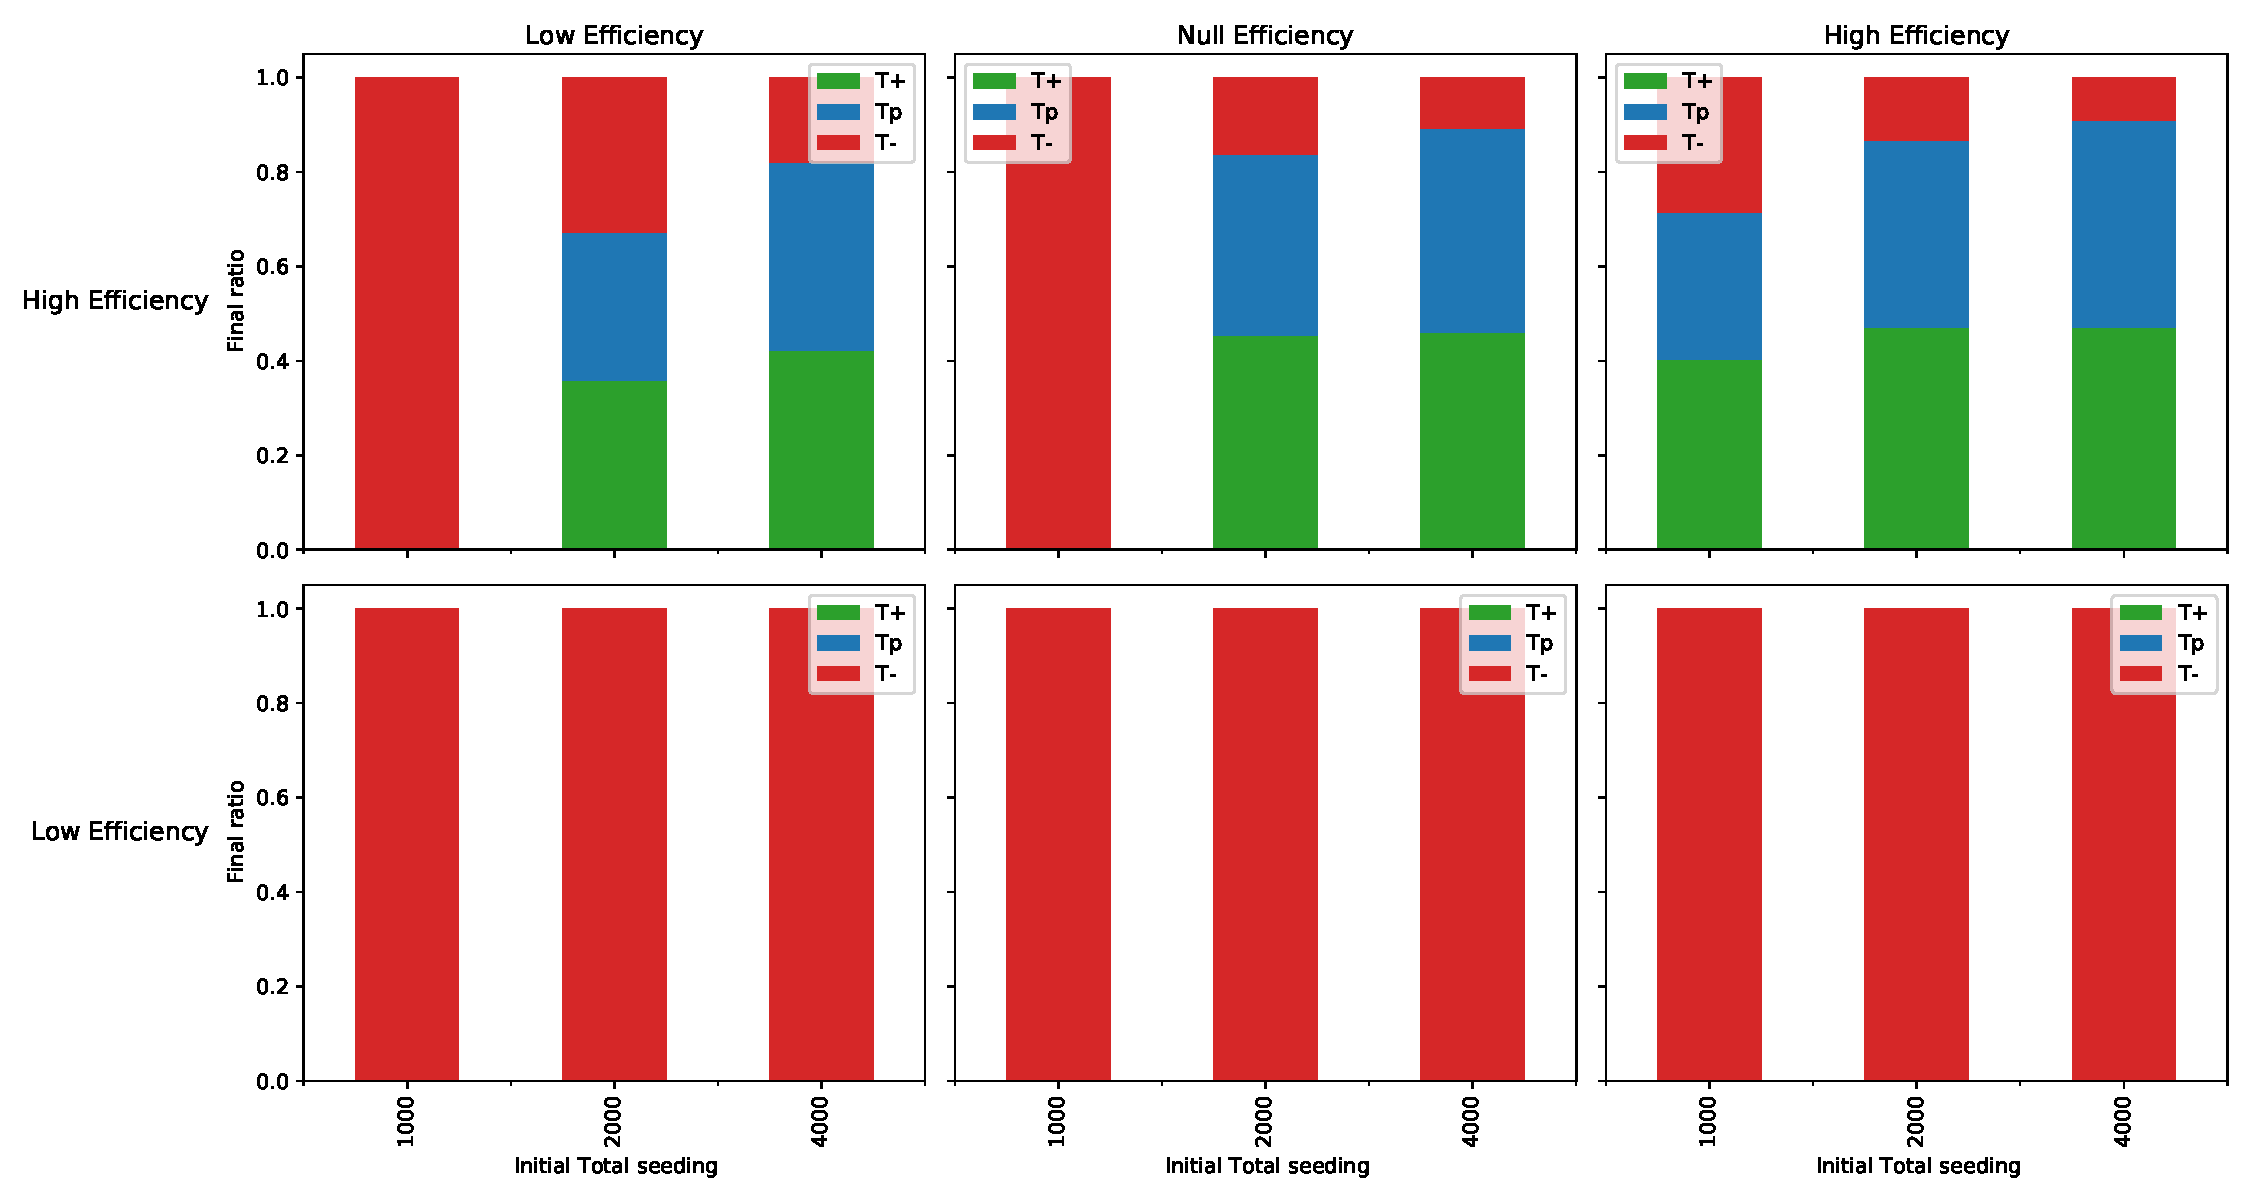
\includegraphics[width=\textwidth]{All3_efficiency_1:1:1}
        \caption{Equal seeding - 1:1:1 }
      \end{subfigure}
      \begin{subfigure}[b]{0.53\textwidth}
        \centering
        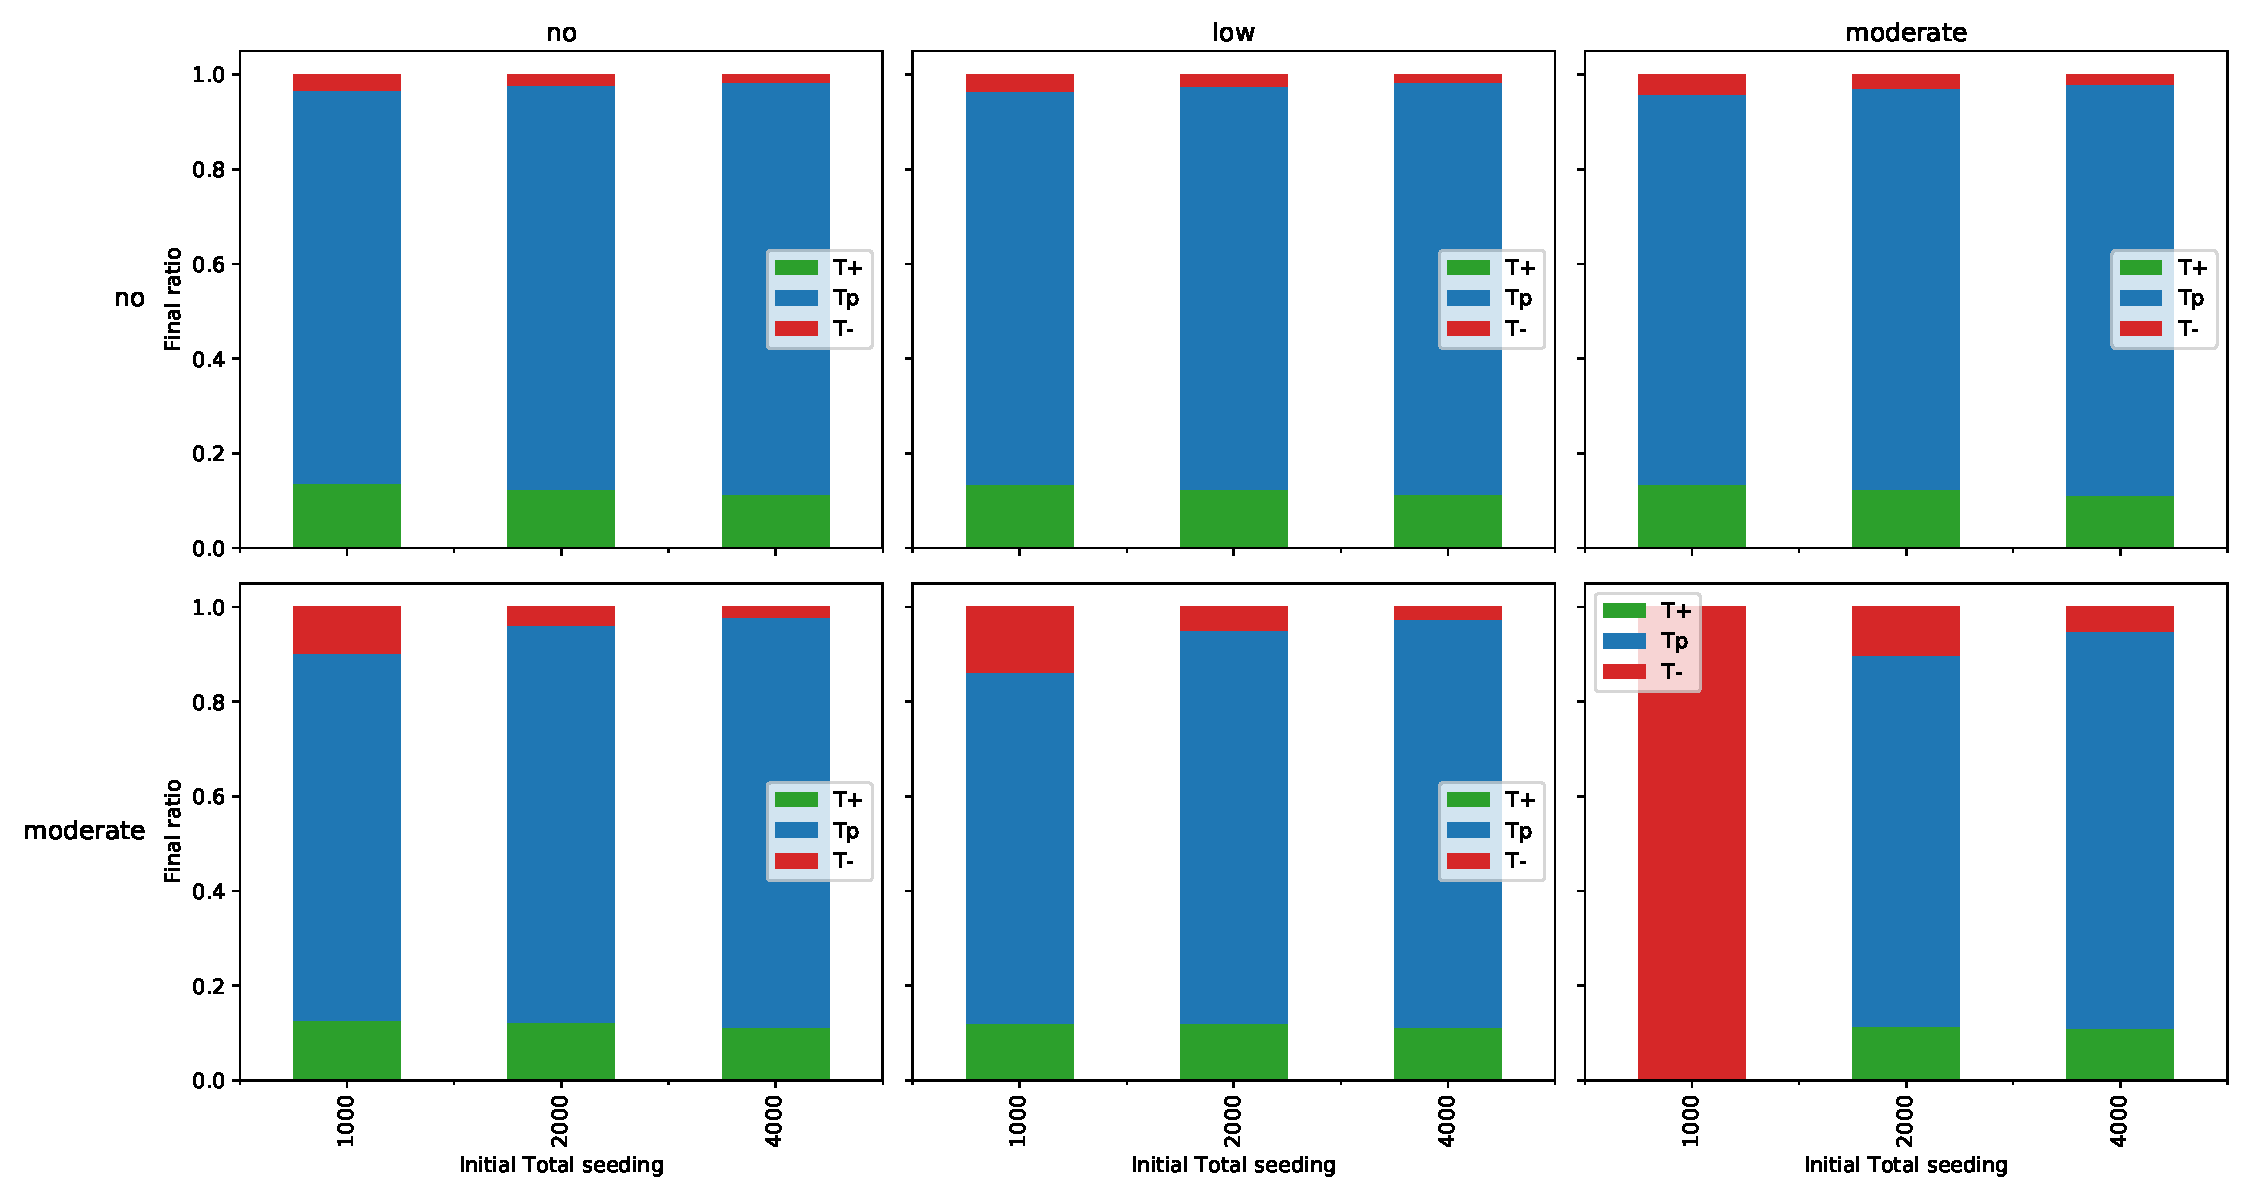
\includegraphics[width=\textwidth]{All3_efficiency_8:1:1}
        \caption{High $T^p$ seeding - 8:1:1}
      \end{subfigure}
    \end{adjustwidth}
    \caption{Final ratio of all cell types. (Stacked bar plot)}
  \end{figure}
  \begin{columns}
    \begin{column}{0.5\textwidth}
      \begin{itemize}
        \item<1-> All the cells have the same limitations
        \item<2-> Higher $T^p$ seeding ratios $\Rightarrow$ increased testosterone production
        \item<3-> Coexistence is important: tumour with $T^p$ and $T^+$ would only respond to therapy
      \end{itemize}
    \end{column}
    \begin{column}{0.5\textwidth}
      \begin{itemize}
        \item<4-> Testosterone: drastic effect on coexistence as only $T^p -T^+$ affected
        \item<5-> Oxygen: minor effect, pushes to extinction if combined limitation on the edge
      \end{itemize}
    \end{column}
  \end{columns}
\end{frame}

\section{What happens when we add therapy?}

\begin{frame}{How is it implemented?}
  \begin{columns}
    \begin{column}{0.43\textwidth}
      \begin{itemize}
        \item<1-> Therapy: modelled as boolean
        \begin{equation}
          \begin{aligned}
            & 1 = \text{MTD}\\
            & 0 = \text{no dose}
          \end{aligned}
        \end{equation}
        \item<2-> Abiraterone:
        blocks $CYP17\alpha$ \\ $T^p$, $T^+$ affected
        \begin{equation}
          p_{test}(abi) = \begin{cases}
          p_{test,max} &\text{if } abi = 0 \\
          p_{test,min} &\text{if } abi = 1 \\
          \end{cases}
          \label{p_test_dose_eq}
        \end{equation}

        \item<3-> Docetaxel: disrupts microtubule \\ All 3 affected
        \begin{equation}
          r_i(dtx) = \begin{cases}
          r_{i,max} &\text{if } dtx = 0 \\
          r_{i,min} &\text{if } dtx = 1 \\
          \end{cases}
          \label{r_dose_eq}
        \end{equation}

      \end{itemize}
    \end{column}
    \begin{column}{0.6\textwidth}
      \begin{itemize}
        \item<4-> SOC\footnotemark[1]: dose given at MTD\footnotemark[1] from the beginning
        \begin{equation}
          dose(y,t) = 1 \quad \forall\ t, y
          \label{dose_soc_eq}
        \end{equation}
        \item<5-> AT\footnotemark[1]: binary mode considered
        \begin{itemize}
          \item Dose at MTD\footnotemark[1] when on
          \item Therapy turned on when population above On threshold
          \item Therapy turned off when population below Off threshold
        \end{itemize}
        \begin{equation}
          dose(y,t) = \begin{cases}
          0 &\text{if } dose(y,t-\Delta t) = 0 \text{ and } y < \text{On} \\
          1 &\text{if } dose(y,t-\Delta t) = 0 \text{ and } y \geq \text{On} \\
          1 &\text{if } dose(y,t-\Delta t) = 1 \text{ and } y > \text{Off} \\
          0 &\text{if } dose(y,t-\Delta t) = 1 \text{ and } y \leq \text{Off} \\
          \end{cases}
          \label{dose_at_eq}
        \end{equation}
      \end{itemize}
    \end{column}
  \end{columns}
  \footnotetext[1]{MTD: Maximum tolerated dose, SOC: Standard-Of-Care, AT: Adaptive Therapy}
  \footnotetext[2]{abi: abiraterone, dtx: docetaxel}
\end{frame}

\begin{frame}{What happens with Standard-Of-Care?}
  \begin{figure}[h]
    \begin{adjustwidth}{-5cm}{-5cm}
      \centering
      \begin{subfigure}[b]{0.53\textwidth}
        \centering
        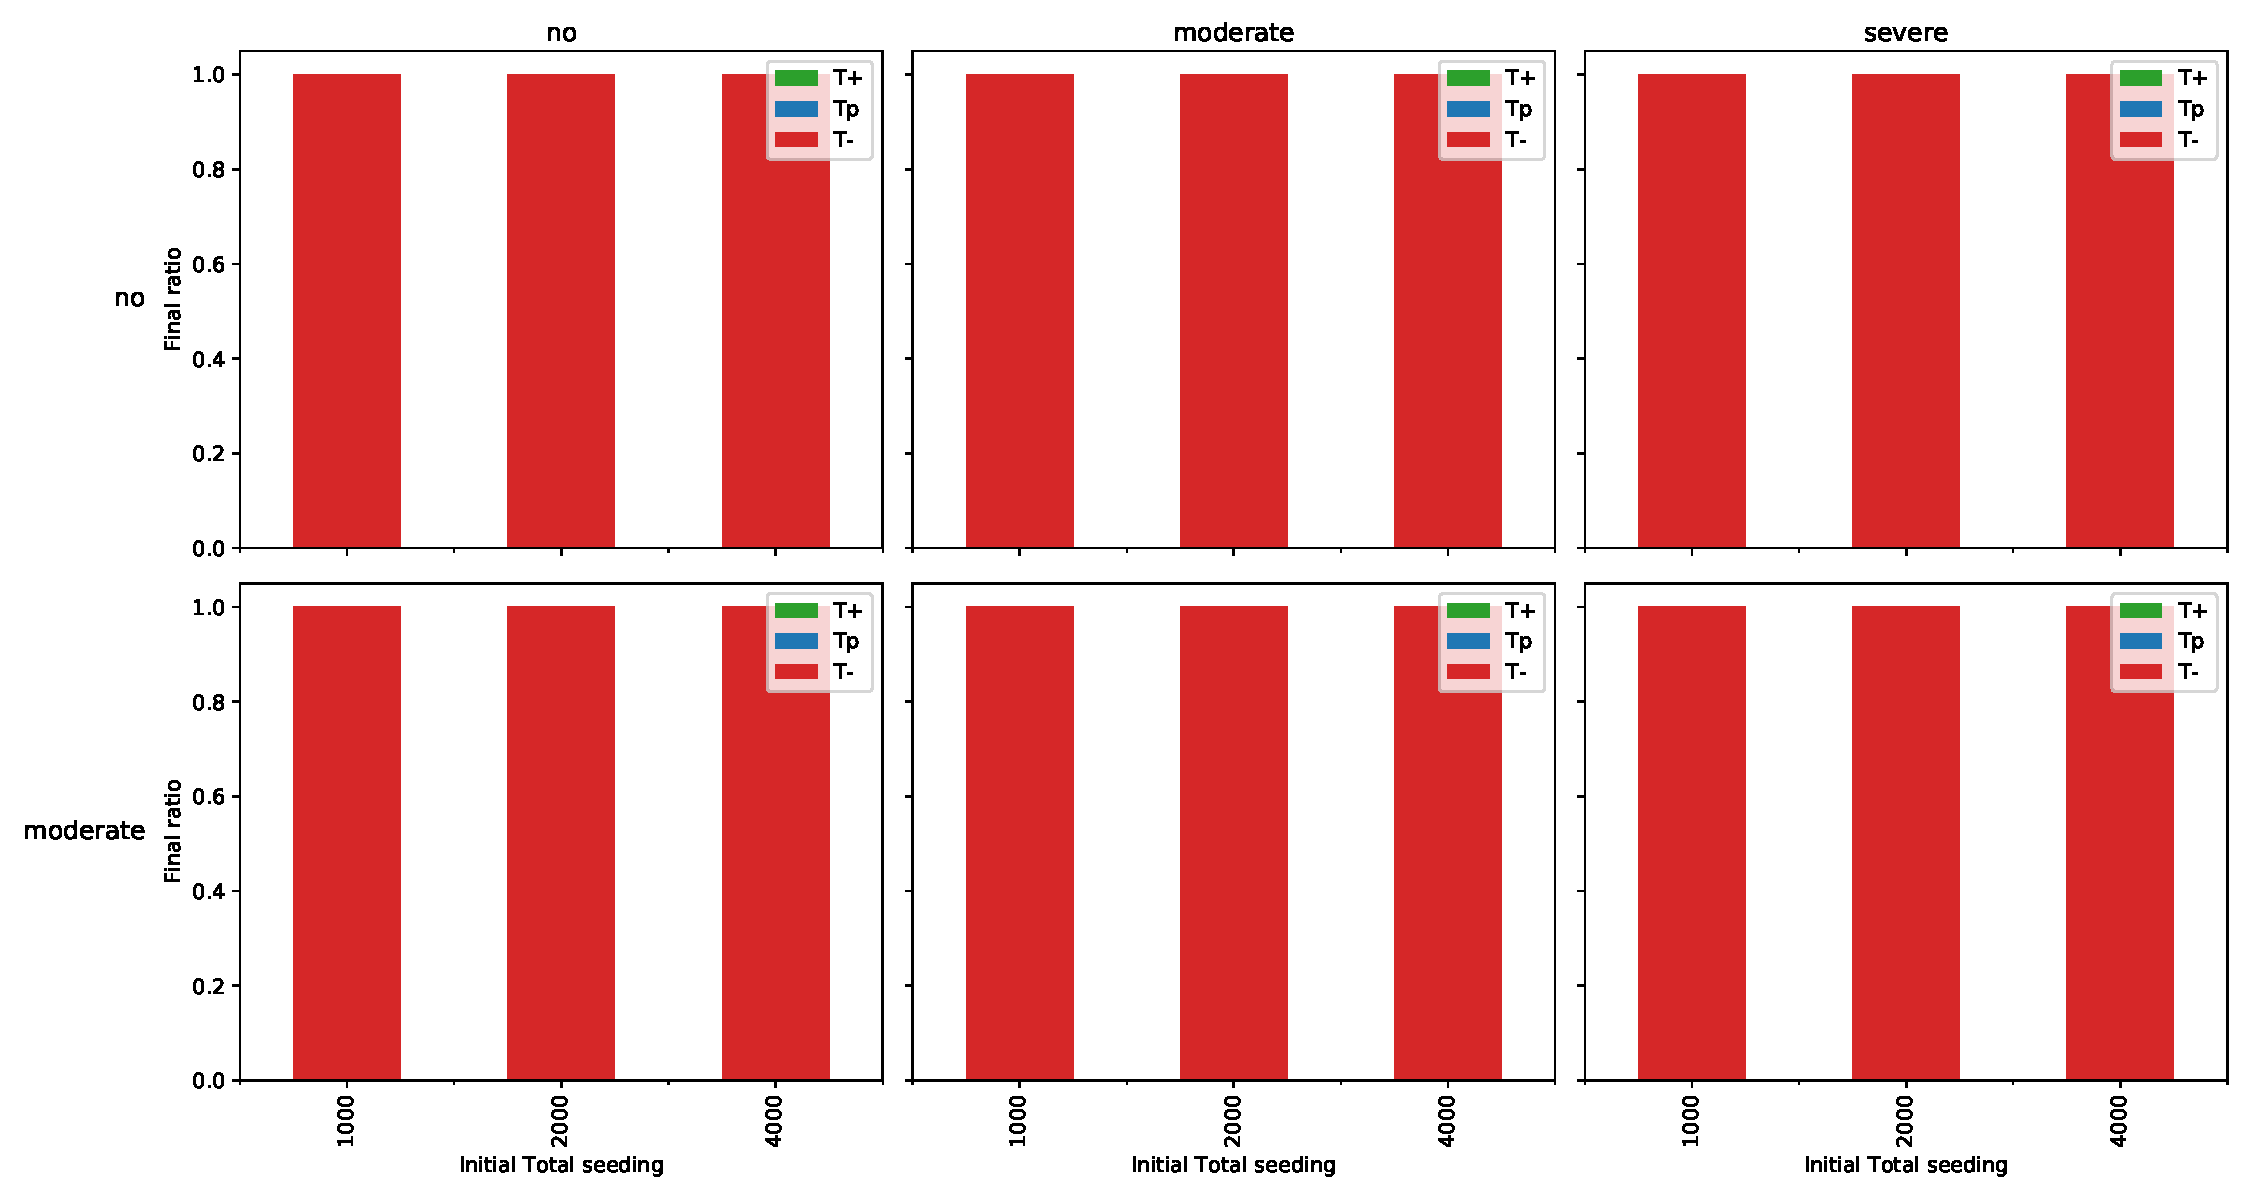
\includegraphics[width=\textwidth]{All3_therapy-SOC_1:1:1}
        \caption{Equal seeding - 1:1:1}
      \end{subfigure}
      \begin{subfigure}[b]{0.53\textwidth}
        \centering
        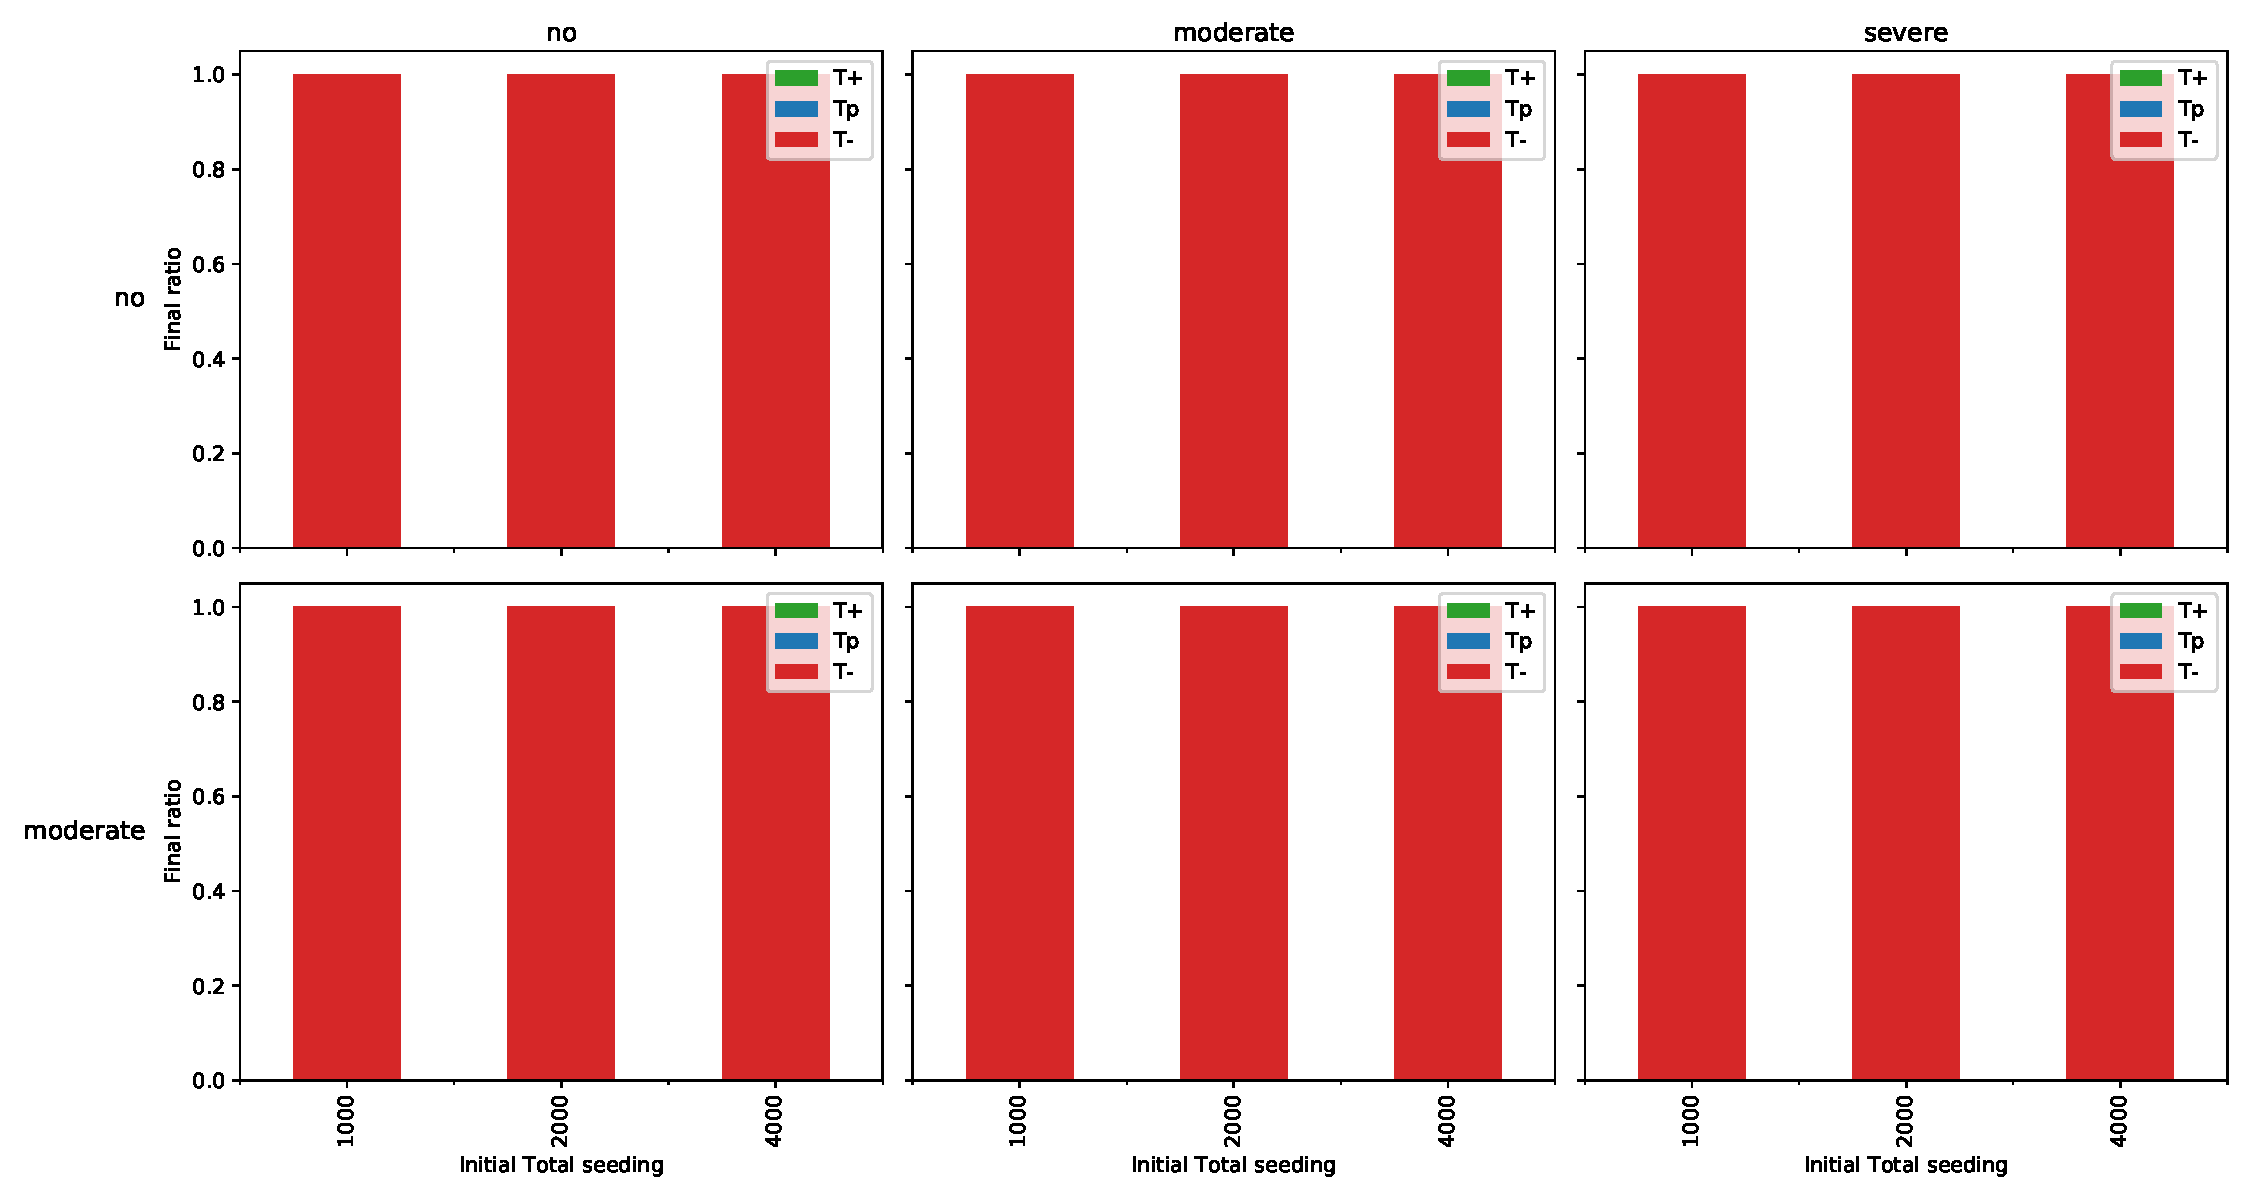
\includegraphics[width=\textwidth]{All3_therapy-SOC_8:1:1}
        \caption{High $T^p$ seeding - 8:1:1}
      \end{subfigure}
    \end{adjustwidth}
    \caption{Final ratio of all cell types under standard-of-care. (Stacked bar plot)}
  \end{figure}
  \begin{columns}
    \begin{column}{0.5\textwidth}
      \begin{itemize}
        \item $T^+, T^p$ go extinct in all cases
      \end{itemize}
    \end{column}
    \begin{column}{0.5\textwidth}
      \begin{itemize}
        \item Testosterone levels insufficient for growth
      \end{itemize}
    \end{column}
  \end{columns}
\end{frame}

\begin{frame}{Thresholds for Adaptive Therapy }
  \begin{figure}[h]
    \centering
    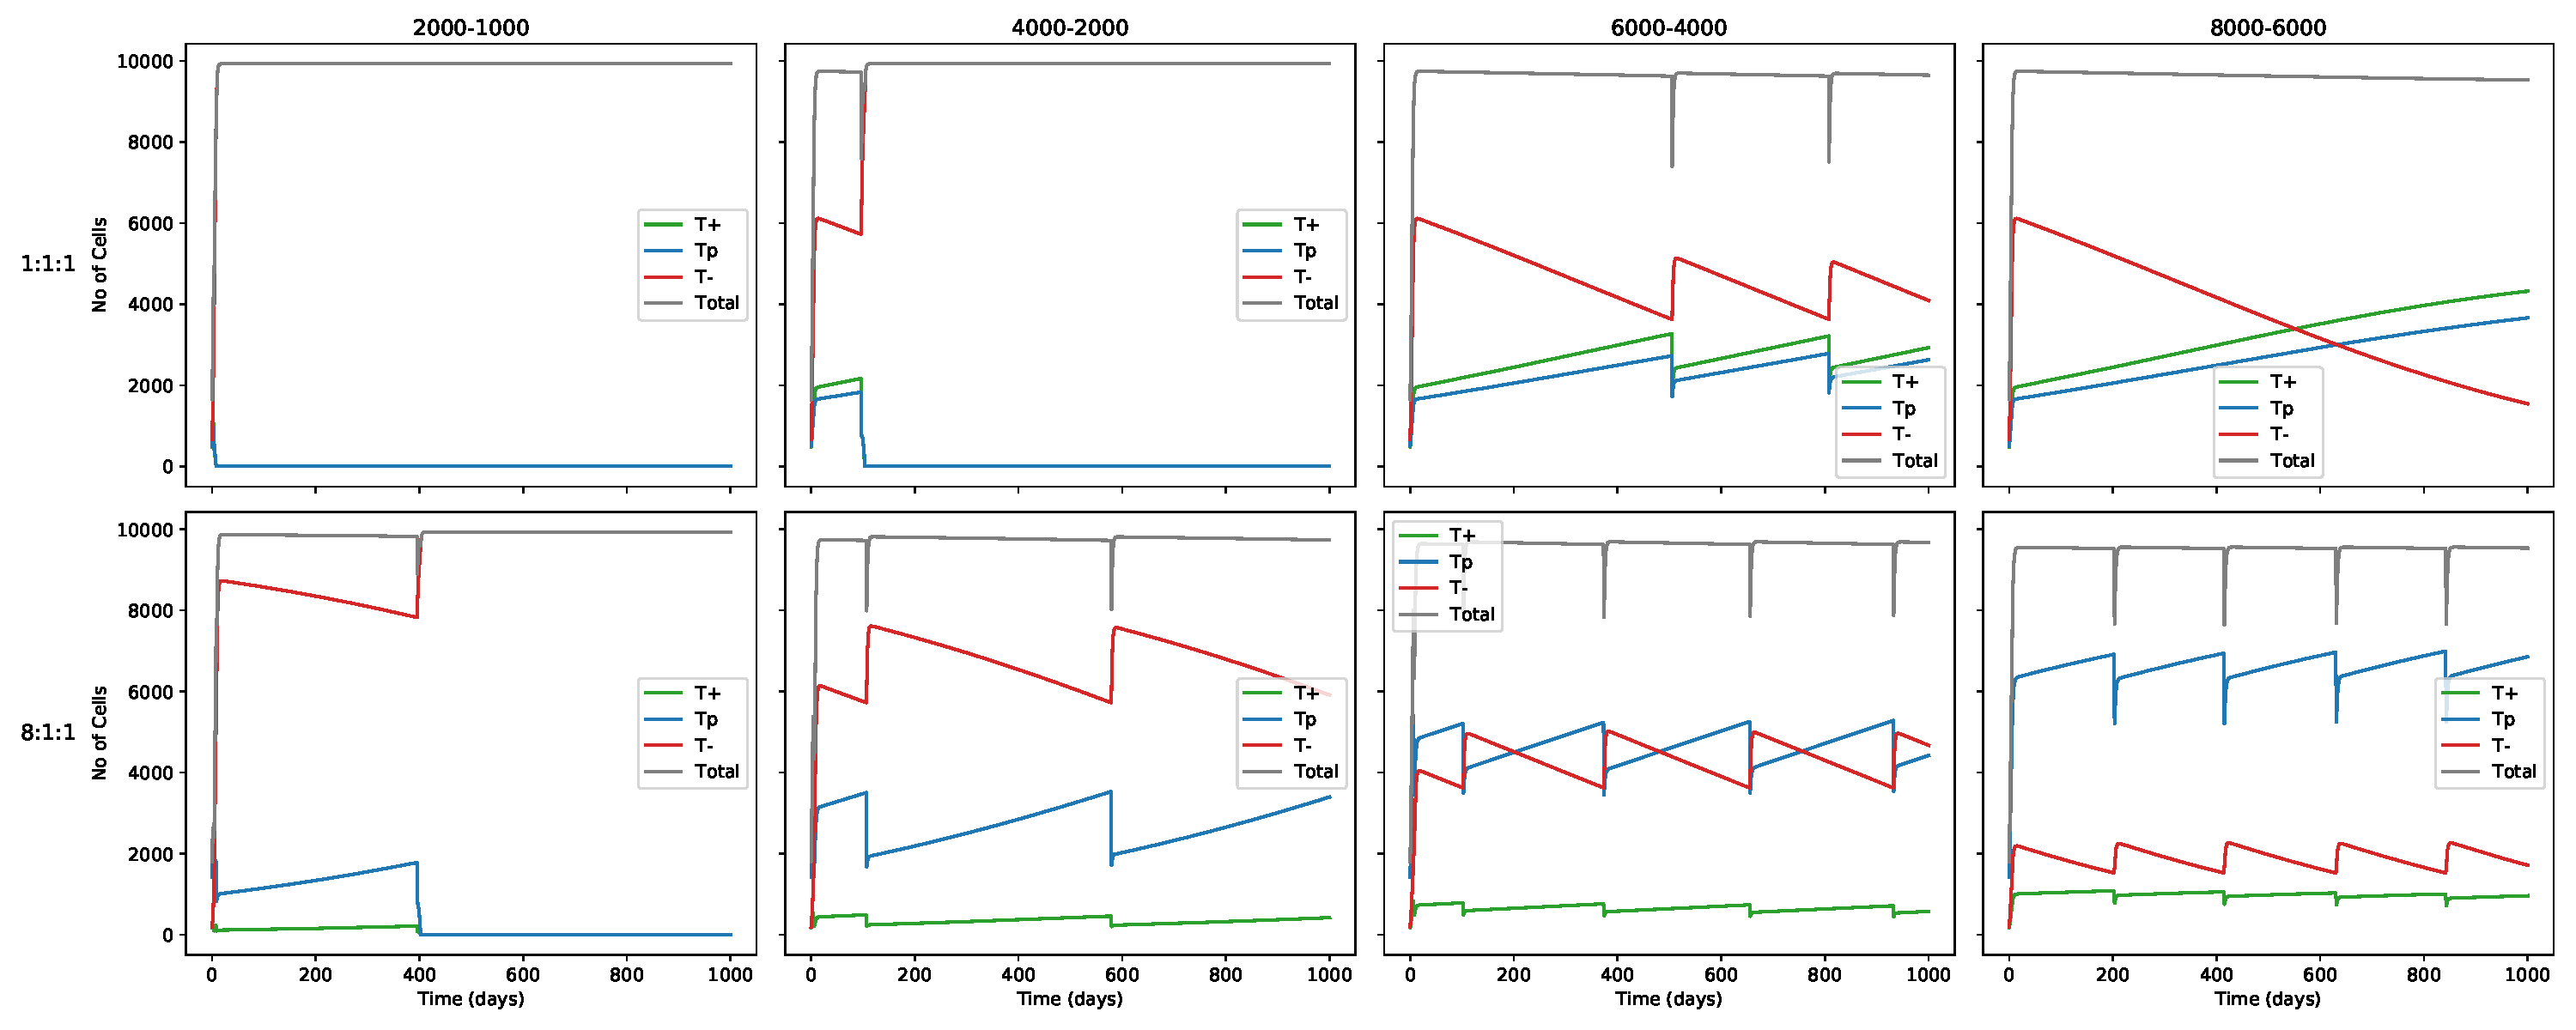
\includegraphics[width=0.7\textwidth]{All3_therapy-standardization}
    \caption{Standardisation of threshold for adaptive therapy}
  \end{figure}
  \begin{columns}
    \begin{column}{0.65\textwidth}
      \begin{itemize}
        \item<1-> Low threshold: $T^-$ inhibits $T^p - T^+$ and causes extinction
        \item<2-> High threshold: $T^+ - T^p$ can compete with $T^-$ \cite{Hansen}
        \item<3-> Too High: No therapy applied as On threshold never crossed
        \item<4-> Chosen- On: 6000, Off: 4000
      \end{itemize}
    \end{column}
    \begin{column}{0.4\textwidth}
      \begin{itemize}
        \item<5-> $T^+ + T^p$ only for threshold
        \item<5-> With total: $T^+ - T^p$ go extinct before therapy turned off
      \end{itemize}
    \end{column}
  \end{columns}
\end{frame}

\begin{frame}{Is Adaptive Therapy better?}
  \begin{figure}[h]
    \begin{adjustwidth}{-5cm}{-5cm}
      \centering
      \begin{subfigure}[b]{0.53\textwidth}
        \centering
        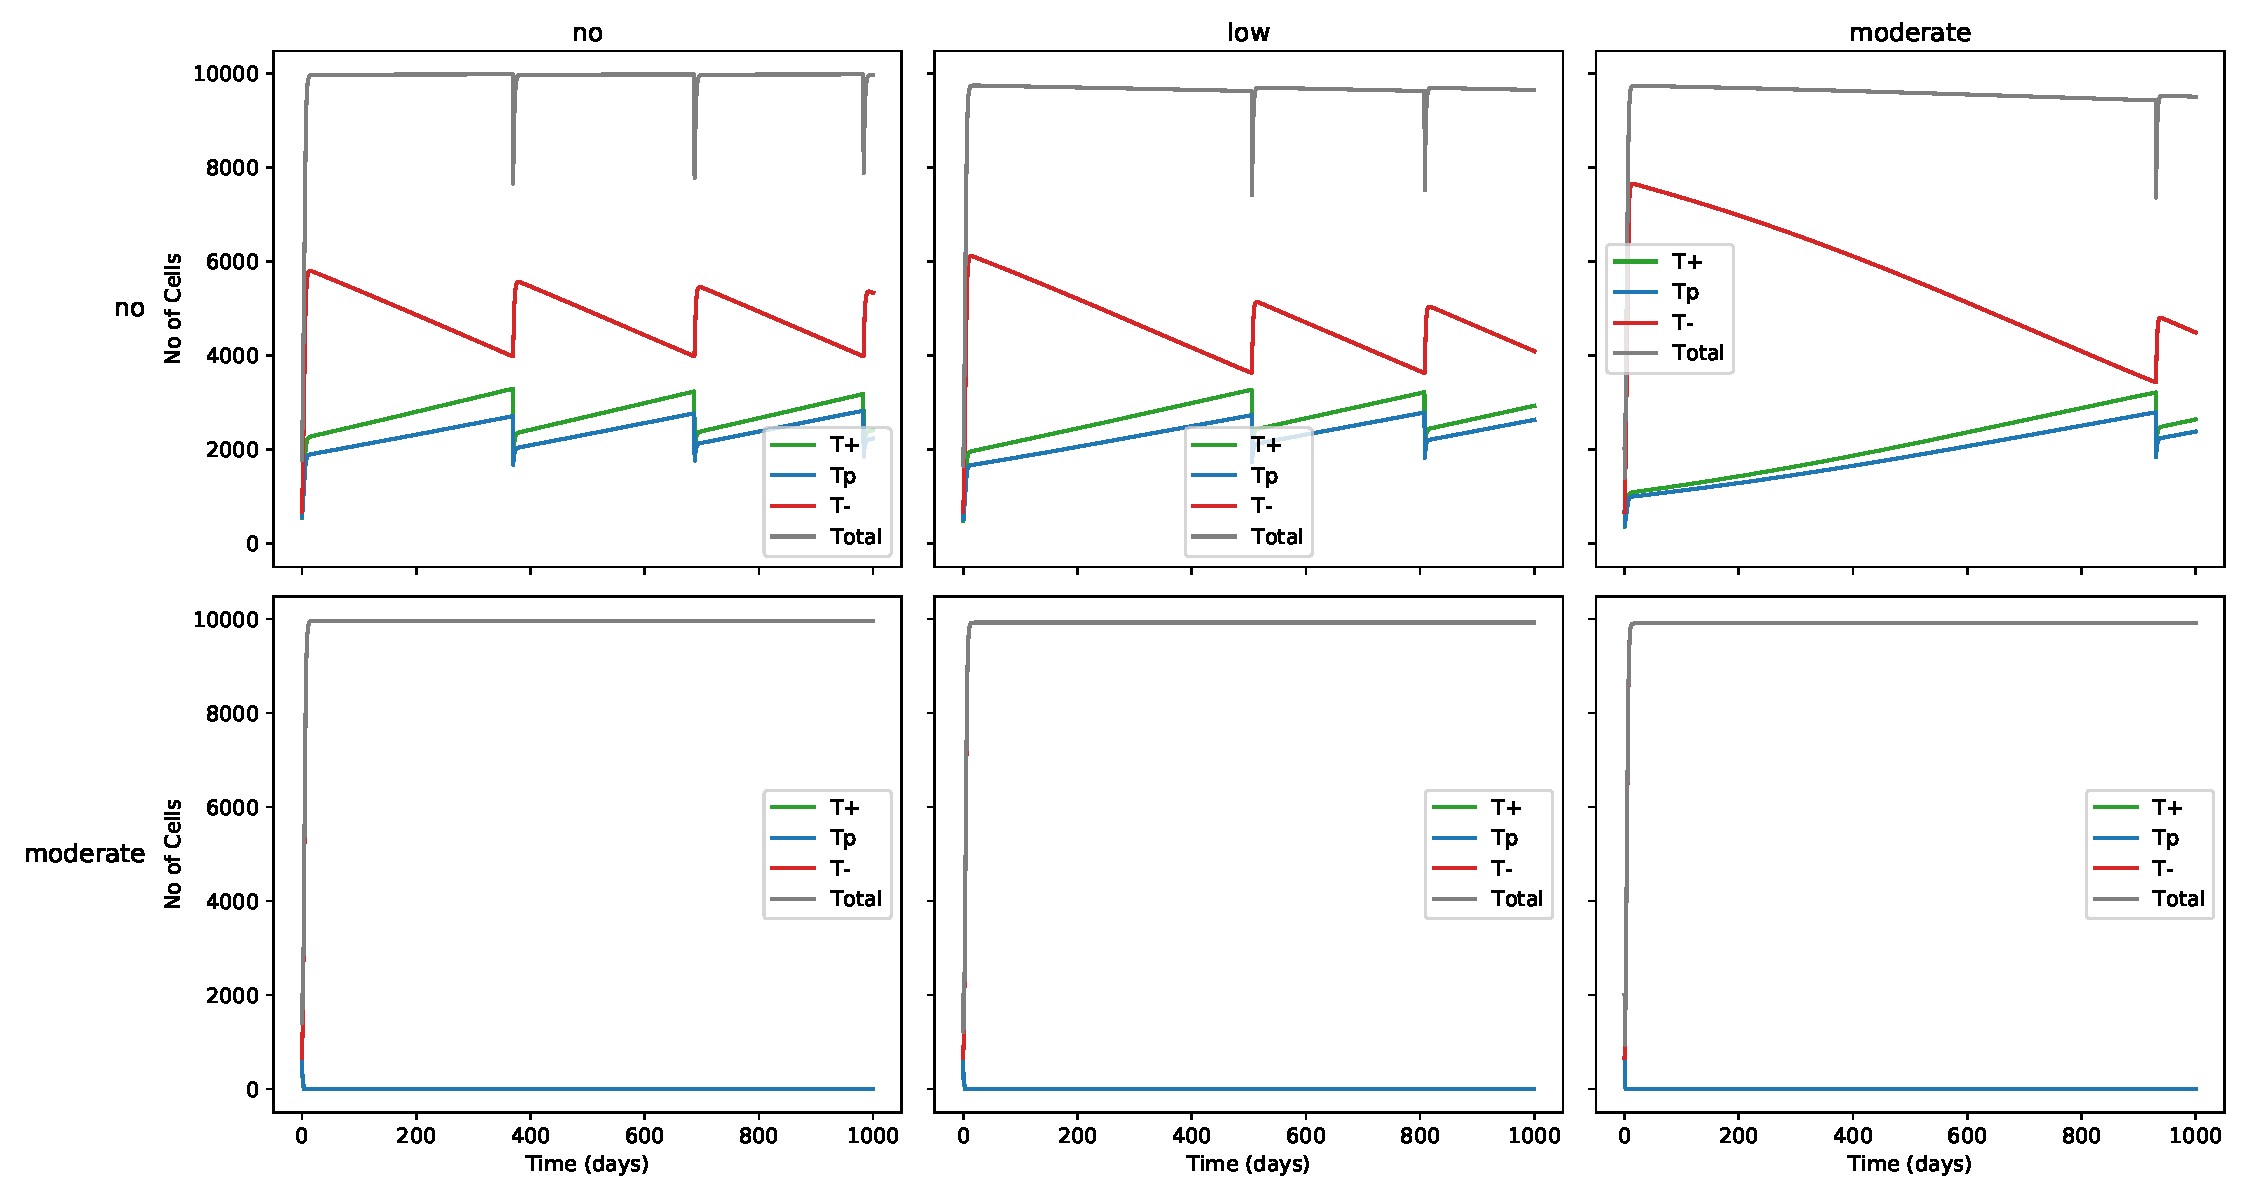
\includegraphics[width=\textwidth]{All3_therapy_1:1:1-2000}
        \caption{Equal seeding - 1:1:1}
      \end{subfigure}
      \begin{subfigure}[b]{0.53\textwidth}
        \centering
        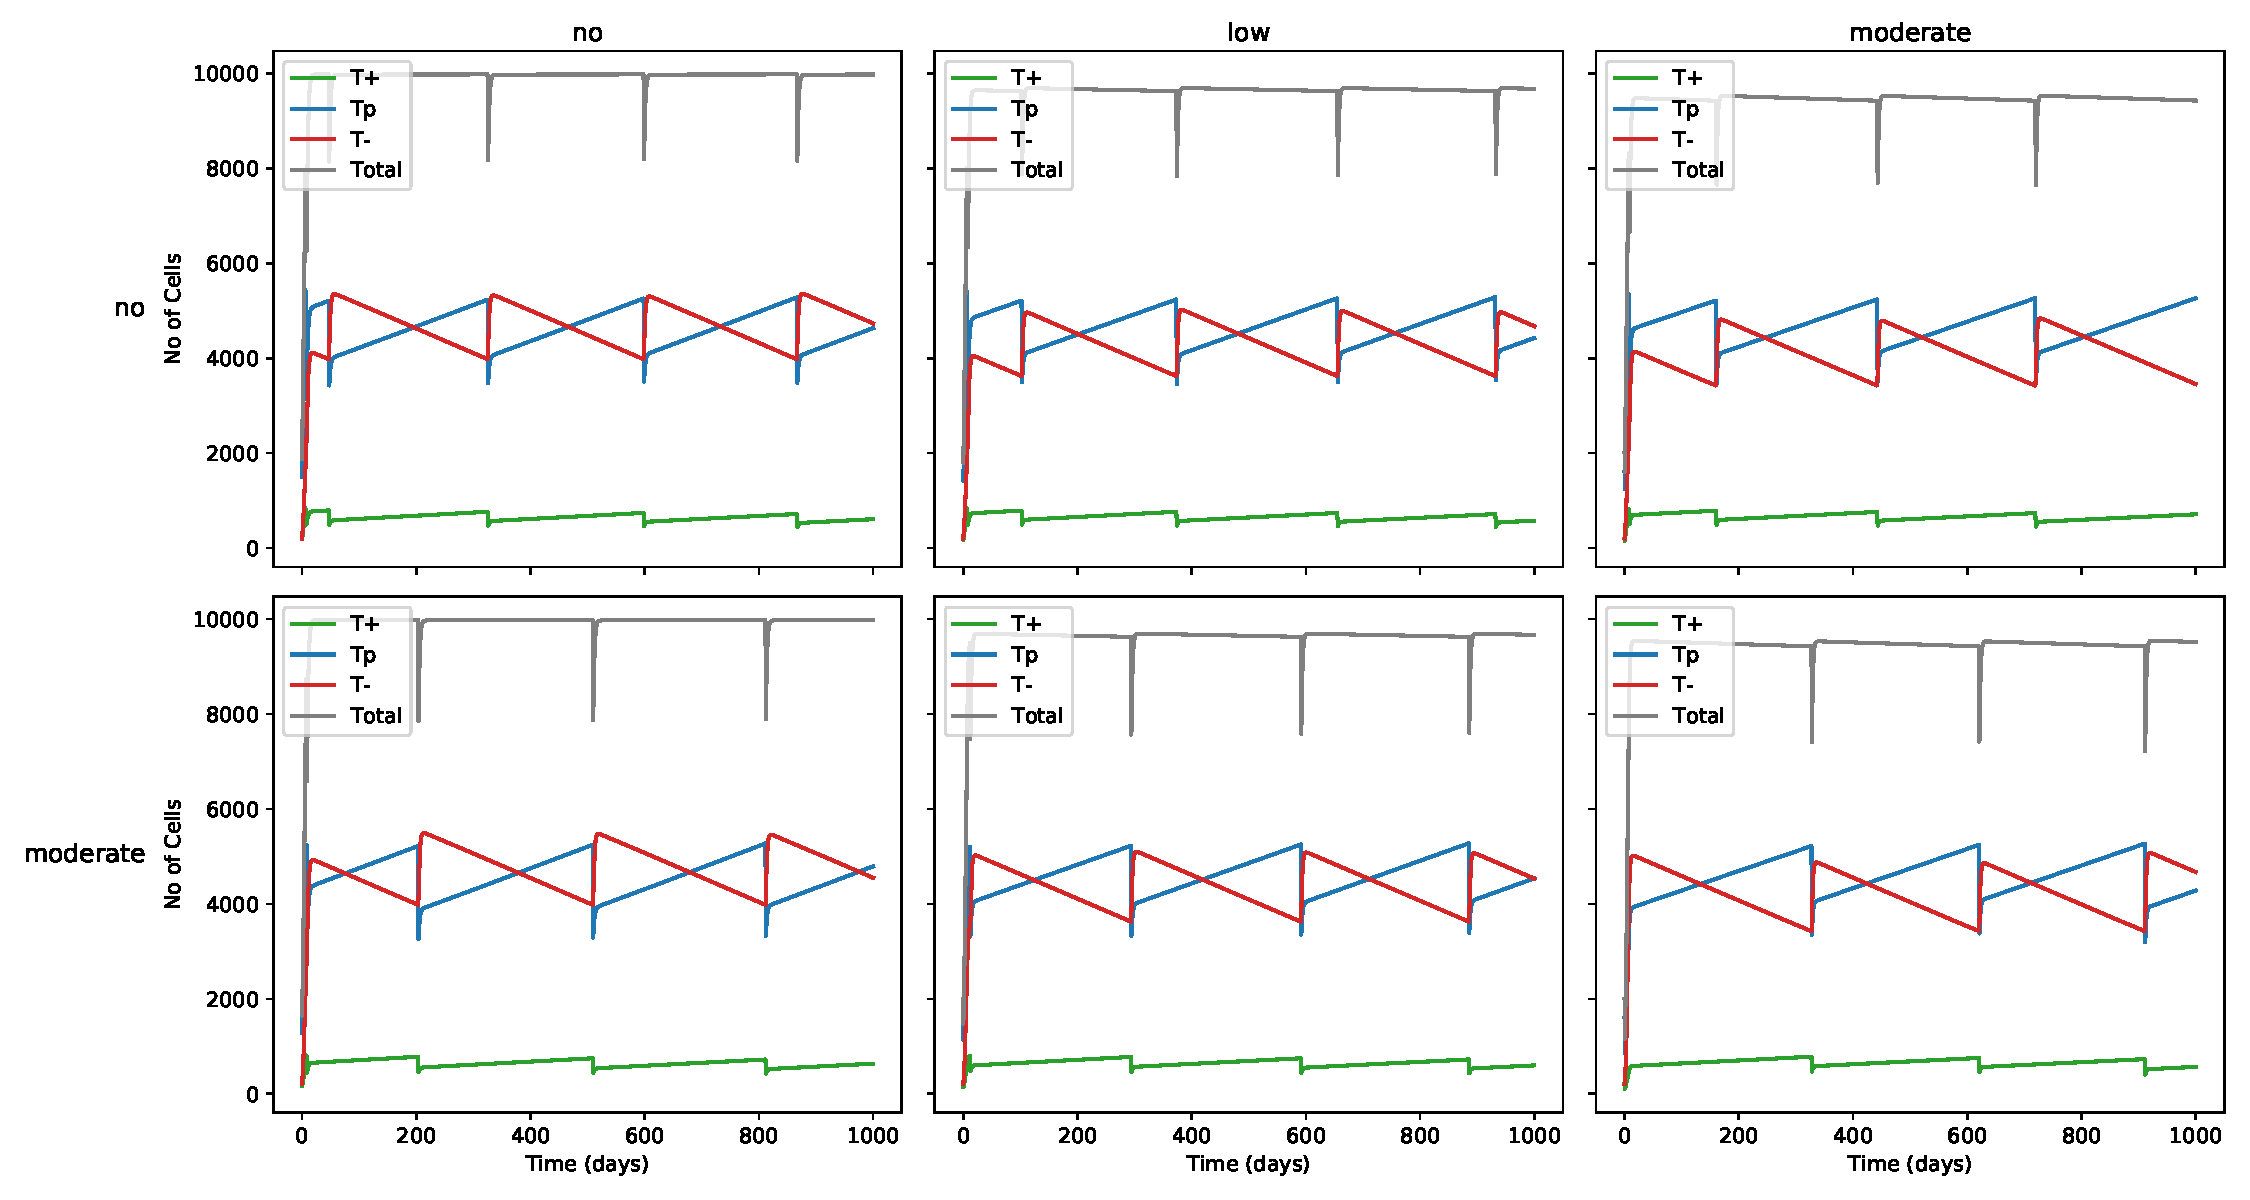
\includegraphics[width=\textwidth]{All3_therapy_8:1:1-2000}
        \caption{High $T^p$ seeding - 8:1:1}
      \end{subfigure}
    \end{adjustwidth}
    \caption{Time-series of all cell types with adaptive therapy. (On:6000, Off:4000)}
  \end{figure}
  \begin{columns}
    \begin{column}{0.5\textwidth}
      \begin{itemize}
        \item<1-> $T^+ - T^p$ extinct just by competition: no effect
        \item<2-> More $T^+ - T^p$ $\rightarrow$ more responsive to abiraterone and better suppress $T^-$
      \end{itemize}
    \end{column}
    \begin{column}{0.5\textwidth}
      \begin{itemize}
        \item<3-> Success of Adaptive therapy:
        \begin{itemize}
          \item<4-> $\checkmark$ Preventing competitive release of resistant
          \item<5-> $\times$ Reducing tumour burden: $T^-$ replace dead cells
        \end{itemize}
      \end{itemize}
    \end{column}
  \end{columns}
\end{frame}

\section{Can adaptive therapy be even made better?}

\begin{frame}{Can delaying treatment help?}
  \begin{figure}[h]
    \begin{adjustwidth}{-5cm}{-5cm}
      \centering
      \begin{subfigure}[b]{0.53\textwidth}
        \centering
        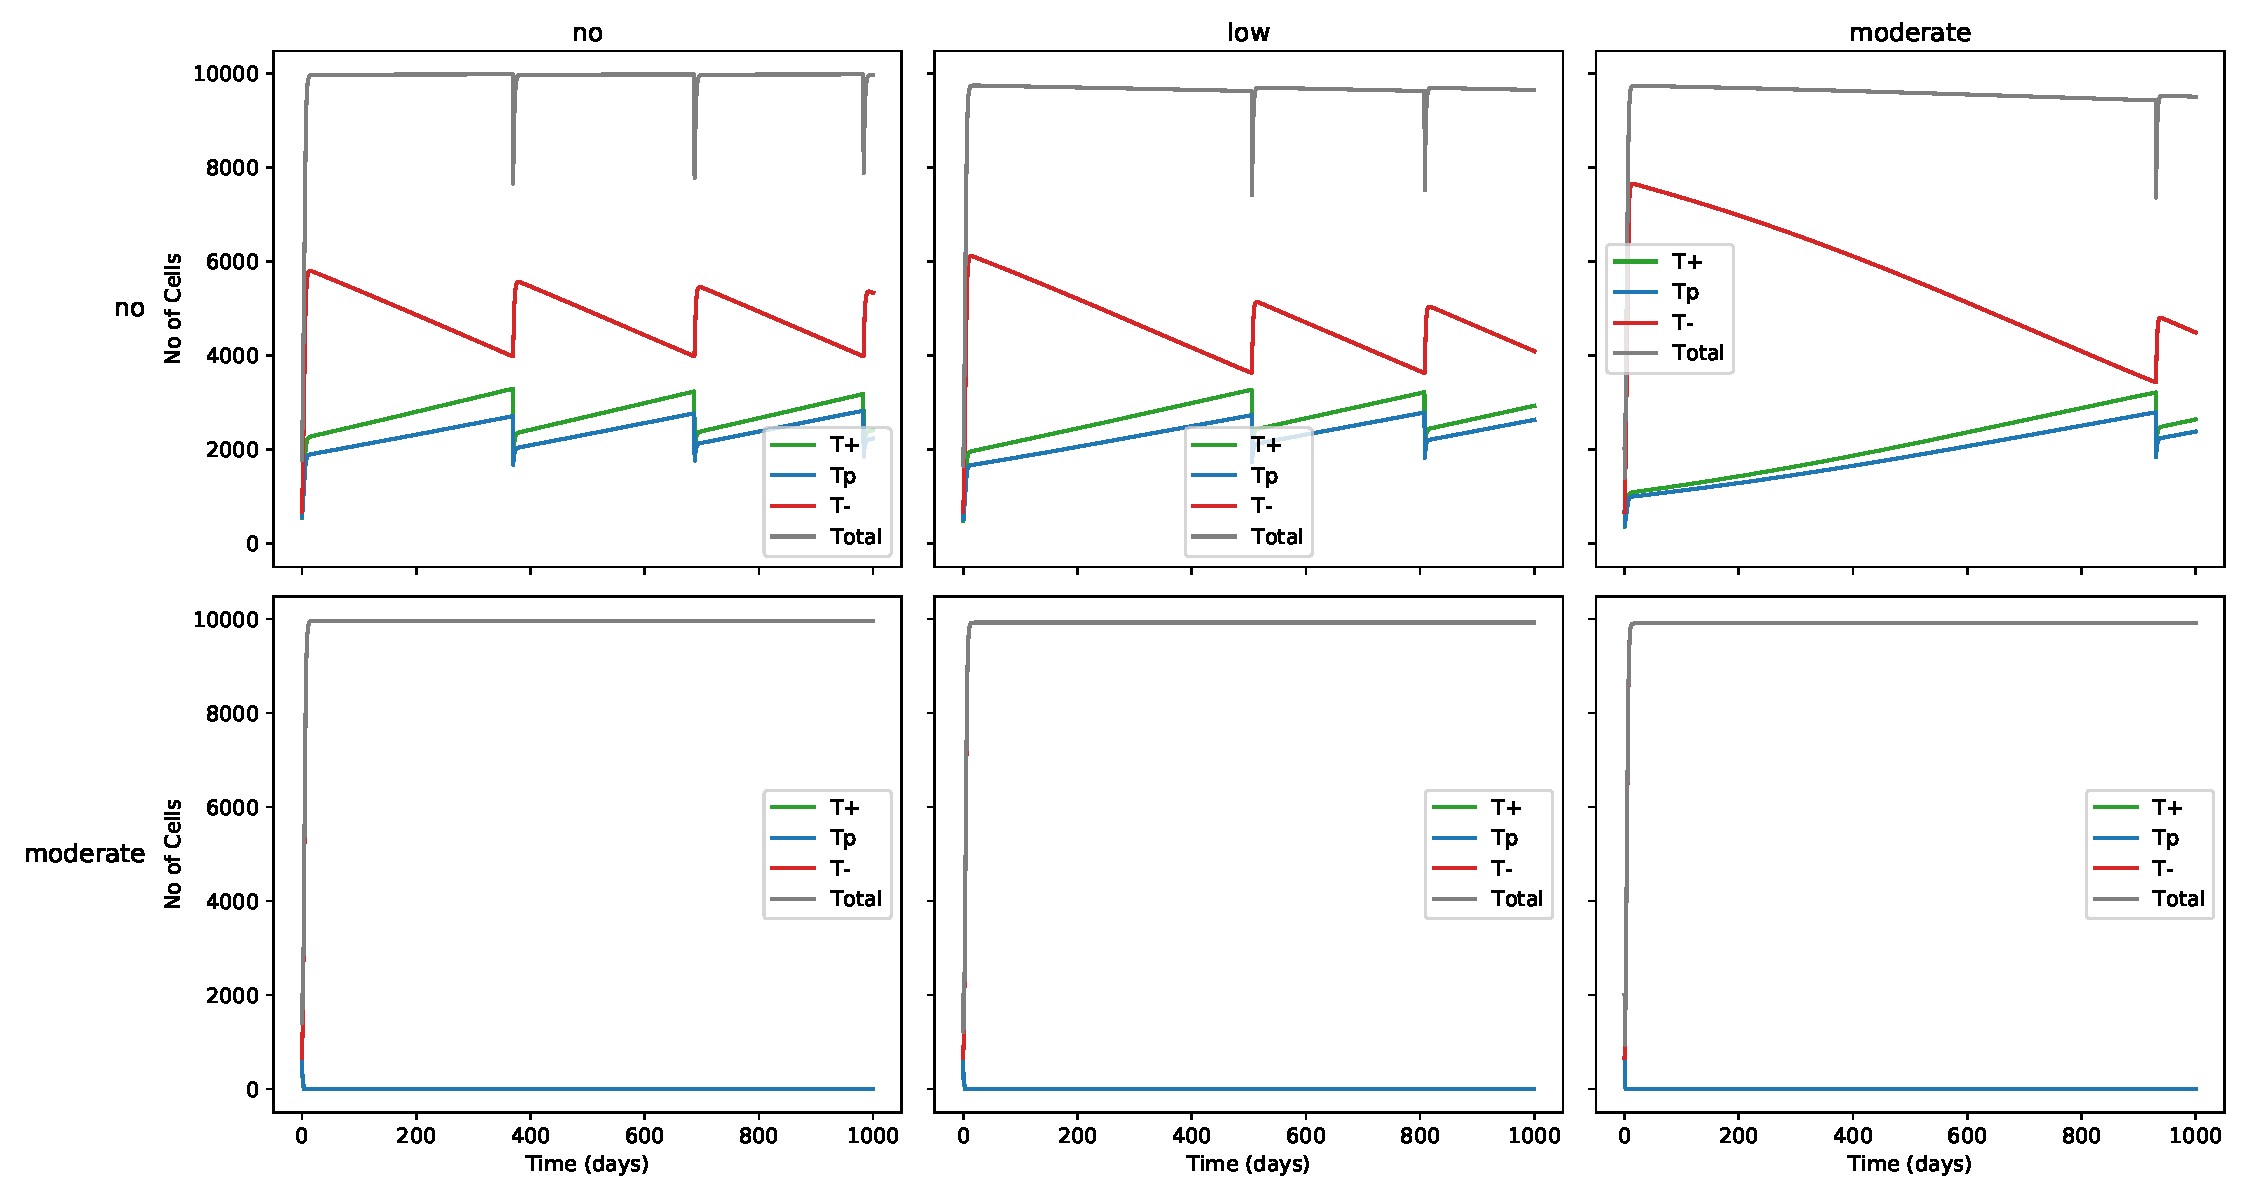
\includegraphics[width=\textwidth]{All3_therapy_200day_1:1:1}
        \caption{Equal seeding - 1:1:1}
      \end{subfigure}
      \begin{subfigure}[b]{0.53\textwidth}
        \centering
        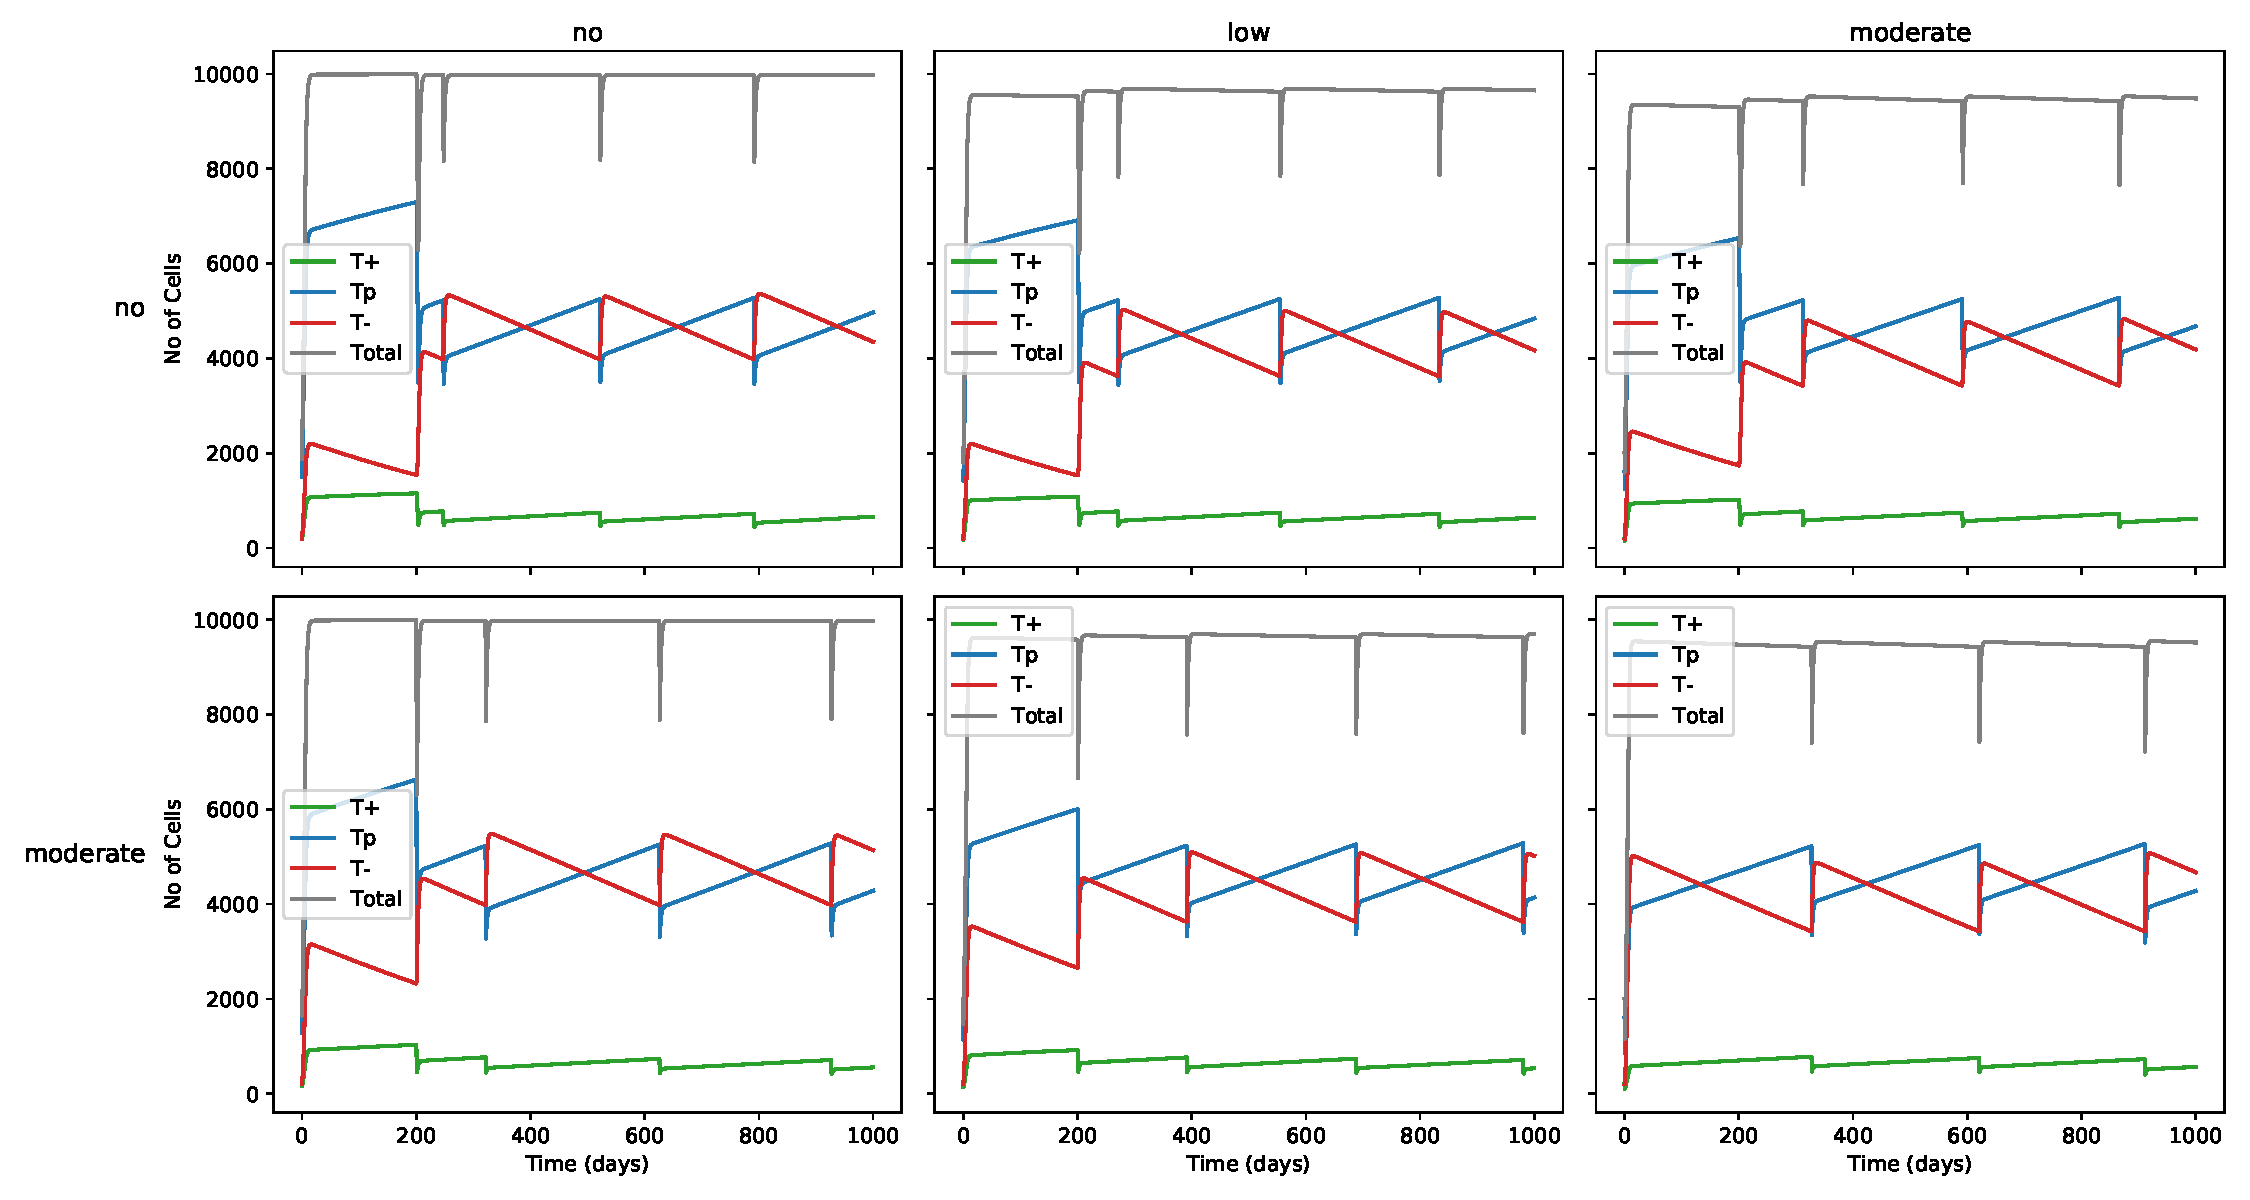
\includegraphics[width=\textwidth]{All3_therapy_200day_8:1:1}
        \caption{High $T^p$ seeding - 8:1:1}
      \end{subfigure}
    \end{adjustwidth}
    \caption{Time-series of all cell types with adaptive therapy delayed by 200 days. (On:6000, Off:4000)}
  \end{figure}
  \begin{columns}
    \begin{column}{0.5\textwidth}
      \begin{itemize}
        \item<1-> $T^+ - T^p$ $\uparrow$ in periods of no therapy
        \item<2-> Speculation: Can delaying bring better balance between $T^+ - T^p$ and $T^-$?
      \end{itemize}
    \end{column}
    \begin{column}{0.5\textwidth}
      \begin{itemize}
        \item<3-> No advantage found as they have similar temporal dynamics
      \end{itemize}
    \end{column}
  \end{columns}
\end{frame}

\begin{frame}{What about using multiple drugs?}
  \begin{figure}[h]
    \begin{adjustwidth}{-5cm}{-5cm}
      \centering
      \begin{subfigure}[b]{0.53\textwidth}
        \centering
        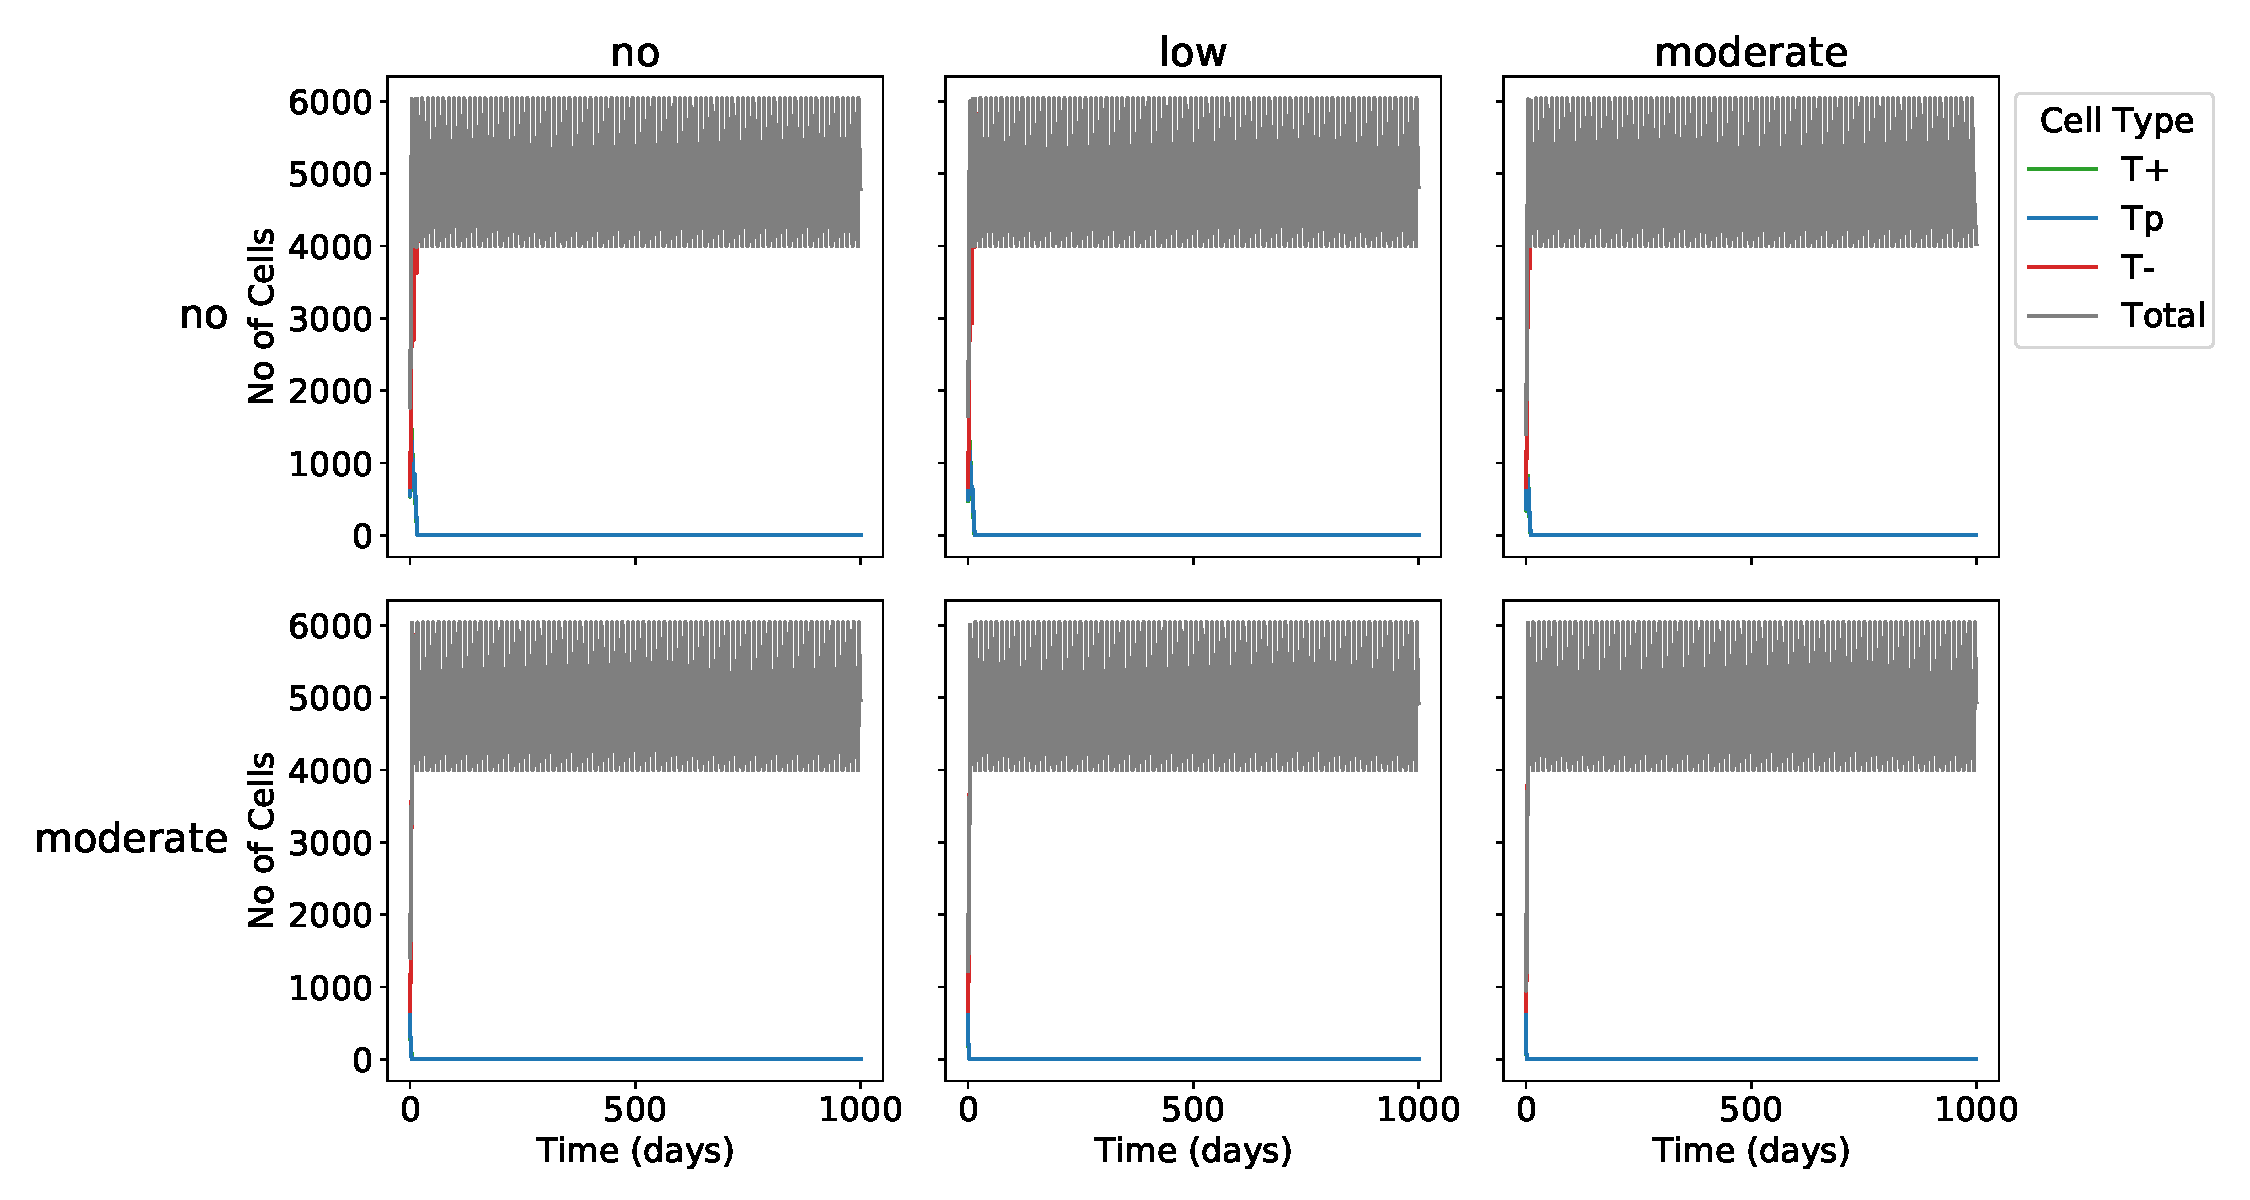
\includegraphics[width=\textwidth]{All3_therapy-combi_1:1:1}
        \caption{Equal seeding - 1:1:1}
      \end{subfigure}
      \begin{subfigure}[b]{0.53\textwidth}
        \centering
        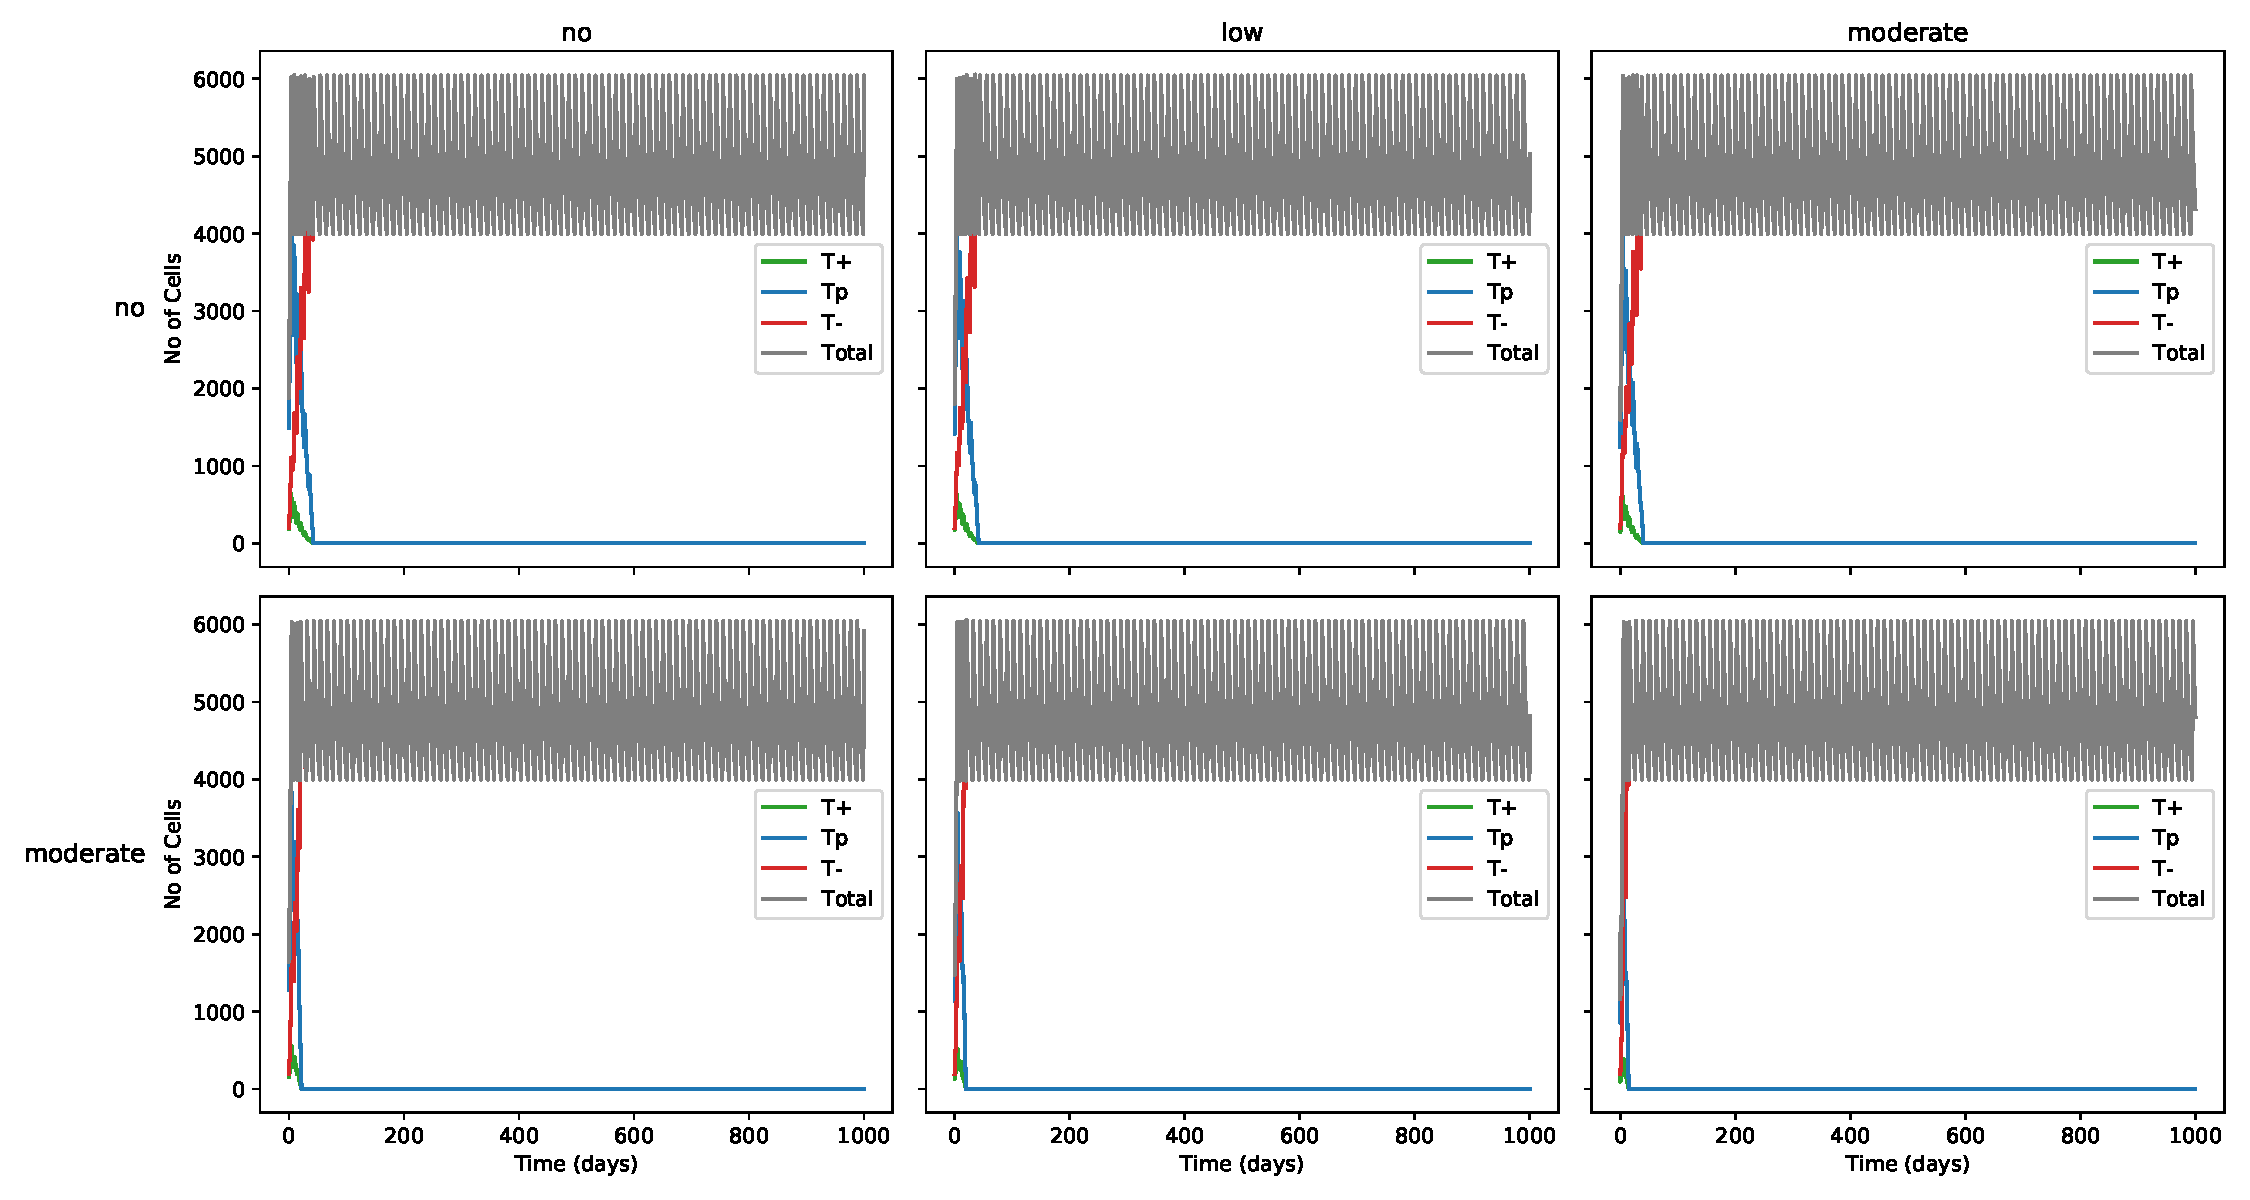
\includegraphics[width=\textwidth]{All3_therapy-combi_8:1:1}
        \caption{High $T^p$ seeding - 8:1:1}
      \end{subfigure}
    \end{adjustwidth}
    \caption{Time-series of all cell types with combination adaptive therapy of abi and dtx\footnotemark[1]. abi(On:6000, Off:4000; $T^+ + T^p$), dtx(On:6000, Off:4000; Total)}
  \end{figure}
  \begin{columns}
    \begin{column}{0.5\textwidth}
      \begin{itemize}
        \item<1-> Hormonal (abi\footnotemark[1]) + cytoxic (dtx\footnotemark[1]) \cite{West}
        \item<2-> Method of action different $\Rightarrow$ Minimal cross resistance
      \end{itemize}
    \end{column}
    \begin{column}{0.5\textwidth}
      \begin{itemize}
        \item<3-> Test-of-concept: would require extensive standardization in future
        \item<4-> $-ve$ effect on coexistence by $\downarrow$ $T^+ - T^p$ outweigh $+ve$ effect on coexistence by $\downarrow$ $T^-$
      \end{itemize}
    \end{column}
  \end{columns}
  \footnotetext[1]{abi: abiraterone, dtx: docetaxel}
\end{frame}


%\chapter{Discussion}
The findings of the study lead to the following points of general interest, beginning with the pairwise interactions. For the $T^p - T^-$ pairwise competition, the limitation of testosterone for $T^p$ and that of oxygen for $T^-$ has a major influence on competition and its outcomes. Increasing the limitation of a given resource for one cell relative to the other leads to the more-limited cell going extinct, regardless of specific identity. Only when the limitations are balanced between two types was coexistence observed. Resource levels can therefore act as control levers of the strength of competitive interactions between cell types and therefore determine the feasibility of coexistence. In addition to resource limitations, the relative initial seeding proportion of the cells can push the outcome in favour of the dominant cell. $T^-$ in conventional terms has an advantage due to its shorter doubling time and the requirement of one less resource. A model that doesn’t account for explicit resource dynamics and limitations might therefore predict that $T^-$ always wins. Although competition coefficients can be made to disfavour $T^-$ , justification for such an artefact isn’t straightforward, particularly compared to the emergence of coexistence we observed in our model due to resource limitation effects.

Similar to $T^p - T^-$, the relative limitation for a given resource of one cell over the other, as well as the relative seeding proportion of the cells, both influence the outcomes of the $T^+ - T^p$ pairwise competition. Resource limitations can in fact be directly compared here unlike $T^p - T^-$, as both the cell types share the same qualitative resource dependencies. $T^p$ has an advantage over $T^+$ with oxygen limitations as the latter requires the former for testosterone. However, with testosterone limitation, $T^p$ has a disadvantage relative to $T^+$ as it would be doubly growth-limited by both testosterone and $T^+$ density. Even though symmetric limitation of a resource across both the cell types produces a similar effect, the difference with testosterone is much more pronounced than with oxygen limitation, possibly indicating a stronger dependence on testosterone for these two cell types.

The general trend discussed above holds for the three-way competition as well. Due to the doubling time advantage of $T^-$ and homogeneous limitations across cell types, testosterone limitations on $T^p$ and $T^+$ have a higher influence on maintaining coexistence between the cells. In this context, it has been possible to identify zones of resource limitation for both testosterone and oxygen where the system goes from coexistence to $T^-$ domination. Strong testosterone limitation without a numerical advantage of higher initial seeding density for $T^p$ leads to $T^-$ domination with no influence from oxygen. Weak testosterone limitation with a numerical advantage for $T^p$ leads to coexistence with no influence of oxygen. Meanwhile, in the other cases where testosterone limitation is intermediate, the outcomes of competition are pushed either towards coexistence or $T^-$ dominance by the oxygen limitation.

This framework used for studying competition alone then helps us understand the outcomes of therapy in mechanistic terms. $T^p$ and $T^+$ are the only cell types to depend on testosterone and hence only they respond to abiraterone. SOC creates an additional limitation of testosterone by reducing the production rates and hence pushes these two cell types to extinction. AT would have no influence where $T^p$ and $T^+$ are pushed to extinction by competition alone and maximum influence when the tumour is dominated by $T^p$ and $T^+$. The resource limitations and seeding proportions therefore have an influence on the success of AT. The success of AT also depends crucially on the therapy window. Higher window would lead to better success, but at the increased physiological cost of maintaining a larger tumour. Meanwhile, with a smaller window achieving control would be more difficult and there would be a higher risk of competitive release. While this mechanistic information makes for a thorough understanding of the system from first principles, it also highlights the gap between the modelling approach and clinical reality. It is clear that application of such ecologically-aware treatment strategies would also require a quantum shift in the nature of information that can be realistically obtained from a cancer patient over meaningful timescales.

Insofar as eliminating the treatment-resistant cell type, all the therapy strategies we tried have been a failure. But, some of this failure has been informative, and it has been possible to avoid or delay competitive release in some cases by maintaining a non-zero population of the responsive cell types $T^+$ and $T^p$. This is broadly in line with current thinking in the field regarding the goals of AT, which are more focused on achieving control than a complete cure. It is worth noting however, that the total tumour burden even when control was achieved was very close to the model’s maximum effective carrying capacity. This could point to an important gap in the conceptualisation of AT that does not include the physiological cost of control over cure. It may then be worth investigating if AT could also be designed to address ways of minimising this cost alongside tumour control.

This study has been an attempt at a proof of concept to illustrate how ecological dynamics within a cancer system can inform progression as well as therapeutic decisions and outcomes. Based on its results so far, the following lines of further development are worth highlighting:
\begin{enumerate}
  \item The exploration of combination therapy in this study has been limited. While the effects of docetaxel in the model were determined based on available experimental data, the ways in which it can be applied are still open modelling questions that can include the frequency of docetaxel, the magnitude of the dose, and the phase shift between abiraterone and docetaxel. Methods of combination therapy other than docetaxel are also known clinically (radiation, steroids, etc) and some of these can be incorporated into the framework of the current model to understand the dynamics of combination therapy better.
  \item The cell types considered here are an oversimplification of actual cells in a biological system, which are highly variable in their functions and phenotypes. Cancer systems in particular can show an even higher degree of such heterogeneity due to their higher mutation rates and genomic instability. Bringing this to bear on the modelling approach I have taken, exploring a heterogeneity of cellular response across cell types to resource availability would be of interest here due to its strong influence on the outcomes of somatic competition and its effect on therapy. This is how pairwise competition has been explored in this study, and its extension to three-way competition should be informative.
  \item In addition to heterogeneity, the cells can also switch their phenotype based on environmental conditions due to phenotypic plasticity. While some theoretical studies have explored the effect of mutational changes within the context of cell competition \cite{Snippert}, phenotypic plasticity remains understudied. It is possible, however, that implementing plasticity or heterogeneous responses would be much easier with an individual based model, which opens up whole new possibilities of exploring the ecological dynamics of the system.
  \item An individual-based model also allows for the addition of spatial heterogeneity to the system, which is an important component of biological variation in cancer populations. Solid tumours in particular have well-known gradients of resources between the tumour core and edge \cite{Fontaine}, which could again open up even more channels of investigation.
\end{enumerate}

These are possible ways in which the current study could be extended and broadened in scope. However, a more general comment on the modelling approach itself is also justified at this point.

Mathematical modelling is a really powerful tool in biology which helps in understanding a system without use of an actual system for the main experimentation. This can be very useful when experimenting on the actual system or biological model is not possible due to ethics, health risks, etc. However, one must keep in mind that all biological models are simplifications and involve many assumptions. Quoting \cite{Box} ``All models are wrong, but some are useful". There are no objective criteria for what makes a good model, or a fair set of prior assumptions. Every model makes assumptions that are manifestations of constraints inherent to the mathematical framework and data availability. What is more important is how these assumptions are structured to enable meaningful study of at least one aspect of the system’s behaviour.

The concept of carrying capacity in a logistic or Lotka-Volterra system is a debated topic and even more so in cancer systems \cite{McLeod,Deisboeck}. Our model also assumes a carrying capacity derived from a rather arbitrary equilibrium value, $y_i^*$, given in \autoref{K_eq}. However, this arbitrariness is partially alleviated since this carrying capacity is not explicitly fixed and instead is dynamically affected by the current concentration of resources. Nevertheless, it still suffers from the same setbacks of any model that invokes a carrying capacity, which is both difficult to define biologically (especially for cancer populations characterised by ``uncontrolled" growth) and usually impossible to separate from the intrinsic growth rate. This leads to the possibility that a modelling approach that does not involve the carrying capacity at all where the resource availability is directly linked to growth rate in a consumer-resource type model may be better suited to study cancer systems that are typically at the edge of resource availability. Furthermore, comparing the differences between such alternate modelling strategies could itself form an informative study of modelling assumptions and their impact on inferences.

The inherently exponential nature of the model made it very sensitive to parameter values and to small fluctuations in environmental conditions. This is borne out particularly clearly in how this system responds to the application of therapy almost instantaneously. The rapidity of these responses could likely hide subtler dynamics that may be more accessible to a different modelling approach that is designed to pick up on them.

Our modelling approach has been more mechanistic in nature than data driven. We have started with parameters from fundamental processes governing the system for the overall behaviour to emerge out of it. A data driven model on the other hand, fits the parameters to clinical data. One could argue that such a data driven model reflects closer to reality since it follows the same dynamics, however, such models don’t give valuable insight into these fundamental processes and act as black boxes. It may then be useful to explore ways of integrating clinical data more closely into mechanistic models, potentially resulting in mechanistic insight that can be applied more directly to clinical practice.


%% Reference styles of Books and research articles are different. Some examples are given below.
\printbibliography
\end{document}
